\documentclass{wber}


\usepackage{amsmath,graphicx,array}
\usepackage{dcolumn,soul}%
\usepackage{amsthm}
\usepackage[figuresright]{rotating}%
\usepackage{algorithm, algorithmicx, algpseudocode}
\usepackage{listings}%
\usepackage[sort]{natbib}
\usepackage{booktabs}
\usepackage[flushleft]{threeparttable}
\usepackage{graphicx}
\usepackage[xetex,colorlinks=true,linkcolor=black,citecolor=black,urlcolor=black]{hyperref}

\bibpunct[, ]{(}{)}{;}{a}{}{,}
\newcommand{\GG}[1]{}
\RequirePackage{url}\def\UrlFont{}


\makeatletter
%%
\def\uns{\ifmmode\,\else$\,$\fi}%
\newtheorem{theorem}{Theorem}
\newtheorem{construction}{Construction}
\newtheorem{estimate}{Estimate}
\newtheorem{lemma}{Lemma}
\newtheorem{corollary}{Corollary}
\newtheorem{result}{Result}
\newtheorem{algth}{Algorithm}
\newtheorem{proposition}{Proposition}
\newtheorem{hypothesis}{Hypothesis}
\newtheorem{experiment}{Experiment}
\newtheorem{definition}{Definition}
\newtheorem{condition}{Condition}
\newtheorem{property}{Property}
\newtheorem{problem}{Problem}
\newtheorem{fact}{Fact}
\newtheorem{assumption}{Assumption}
\newtheorem{eexample}{Example}
\newtheorem{model}{Model}
%%
\makeatother
 
\raggedbottom

\newcommand{\mco}[1]{\multicolumn{1}{c}{#1}}
\newcommand{\mct}[1]{\multicolumn{2}{c}{#1}}

% Redefine the \appendix command
\usepackage{titlesec}
\usepackage{chngcntr} % Package to change the counter

% Define a new counter for the appendix sections
\newcounter{appendixsection}
\newcommand{\appsection}[1]{
    \stepcounter{appendixsection}
    \section*{Appendix A\arabic{appendixsection}: #1}
    \addcontentsline{toc}{section}{Appendix A\arabic{appendixsection}: #1}
    \setcounter{figure}{0} % Reset figure counter for each appendix section
    \setcounter{table}{0} % Reset table counter for each appendix section
    \renewcommand{\thefigure}{A\arabic{appendixsection}.\arabic{figure}} % Custom figure numbering
    \renewcommand{\thetable}{A\arabic{appendixsection}.\arabic{table}} % Custom table numbering
    \renewcommand{\theHfigure}{\thefigure} % Ensure unique hyperlink targets for figures
    \renewcommand{\theHtable}{\thetable} % Ensure unique hyperlink targets for tables
}

\begin{document}

\dhead{Article}

\title{Impact of Twin Lockdowns on Hunger, Labor Market Outcomes, and
Household Coping Mechanisms: Evidence from Uganda}

\author{Claus C. Pörtner} 

\author{Shamma A. Alam}

\author{Ishraq Ahmed}

\affil{Claus C.\ Pörtner (corresponding author) is an associate professor at the
Department of Economics, Seattle University, Seattle, WA, and an
external affiliate at the Center for Studies in Demography and Ecology,
University of Washington, Seattle, WA (email: cportner@seattleu.edu)}

\affil{Shamma A.\ Alam is an associate professor at the Department of Economics,
Dickinson College, Carlisle, PA (email: alams@dickinson.edu)}

\affil{Ishraq Ahmed is a senior economist at the Office of Tax Policy, Virginia
Department of Taxation, VA (email: Ishraq.Ahmed@tax.virginia.gov)}

\affil{We would like to thank seminar participants at Howard University, Alex
Henke, four anonymous referees, and the Editor for their helpful
comments and suggestions. We would also like to thank Pascal Ntaganda
for his research assistance. Partial support for this research came from
a Eunice Kennedy Shriver National Institute of Child Health and Human
Development research infrastructure grant, 5R24HD042828, to the Center
for Studies in Demography and Ecology at the University of Washington. A
supplementary online appendix is available with this article at the
World Bank Economic Review website. R code and text for this article are
available at 
\href{https://github.com/population-research/uganda-covid.git}{github.com/population-research/uganda-covid.git}}

\abstract[Abstract]{
Uganda had two of the strictest COVID-19 lockdowns in
Sub-Saharan Africa. These severe lockdowns provide a unique case study
for understanding the implications of such public health measures on
economic well-being. We use longitudinal data to examine the lockdowns'
short- and medium-term impacts on household food insecurity, labor
market outcomes, and coping strategies. Lockdowns significantly
exacerbated food insecurity immediately and continued to do so in the
medium term. The effect was more pronounced after the second lockdown,
likely from a combination of reduced resilience after the first lockdown
and lower-than-normal rainfall immediately before. There were
substantial decreases in income from various sources---including
agriculture, non-farm businesses, and wage employment---contributing to
the heightened food insecurity. Notably, agricultural households were
less adversely affected, and there was a significant switch to
agricultural activities as a coping mechanism. The other coping
mechanisms households typically rely on for idiosyncratic shocks, such
as remittances and government assistance, failed, contributing to the
sizeable increase in food insecurity.}

\jelcode{I18, I3, J20, J43, O10} 

\keywords{Public health, Food security, COVID-19, Panel data, High-frequency phone surveys, Economic well-being}

\maketitle

\section{Introduction}\label{introduction}

Uganda had two of the strictest COVID-19 lockdowns in Sub-Saharan
Africa, with the most severe parts of these lockdowns covering April
through June 2020 and June through July 2021
\citep{BBC2020, Birner2021, Mahmud2021}. 
Uganda also experienced substantially higher food insecurity during or 
immediately following these lockdowns than at any other time during the 
pandemic as Figure \ref{fig:raw-insecurity} shows.\footnote{The
  definitions of the three levels of food insecurity are described in
  detail below \citep{FAO2015}.} Using longitudinal household data, this
paper aims to understand the extent to which these changes arose from
the twin lockdowns in Uganda by examining food insecurity, labor market
outcomes, income changes, and how households attempted to cope with the
lockdowns.

\begin{figure}
\caption{Food insecurity by survey round of the Uganda high-frequency
phone survey on COVID-19 together with severe lockdown periods
shaded}\label{fig:raw-insecurity}
\begin{center}
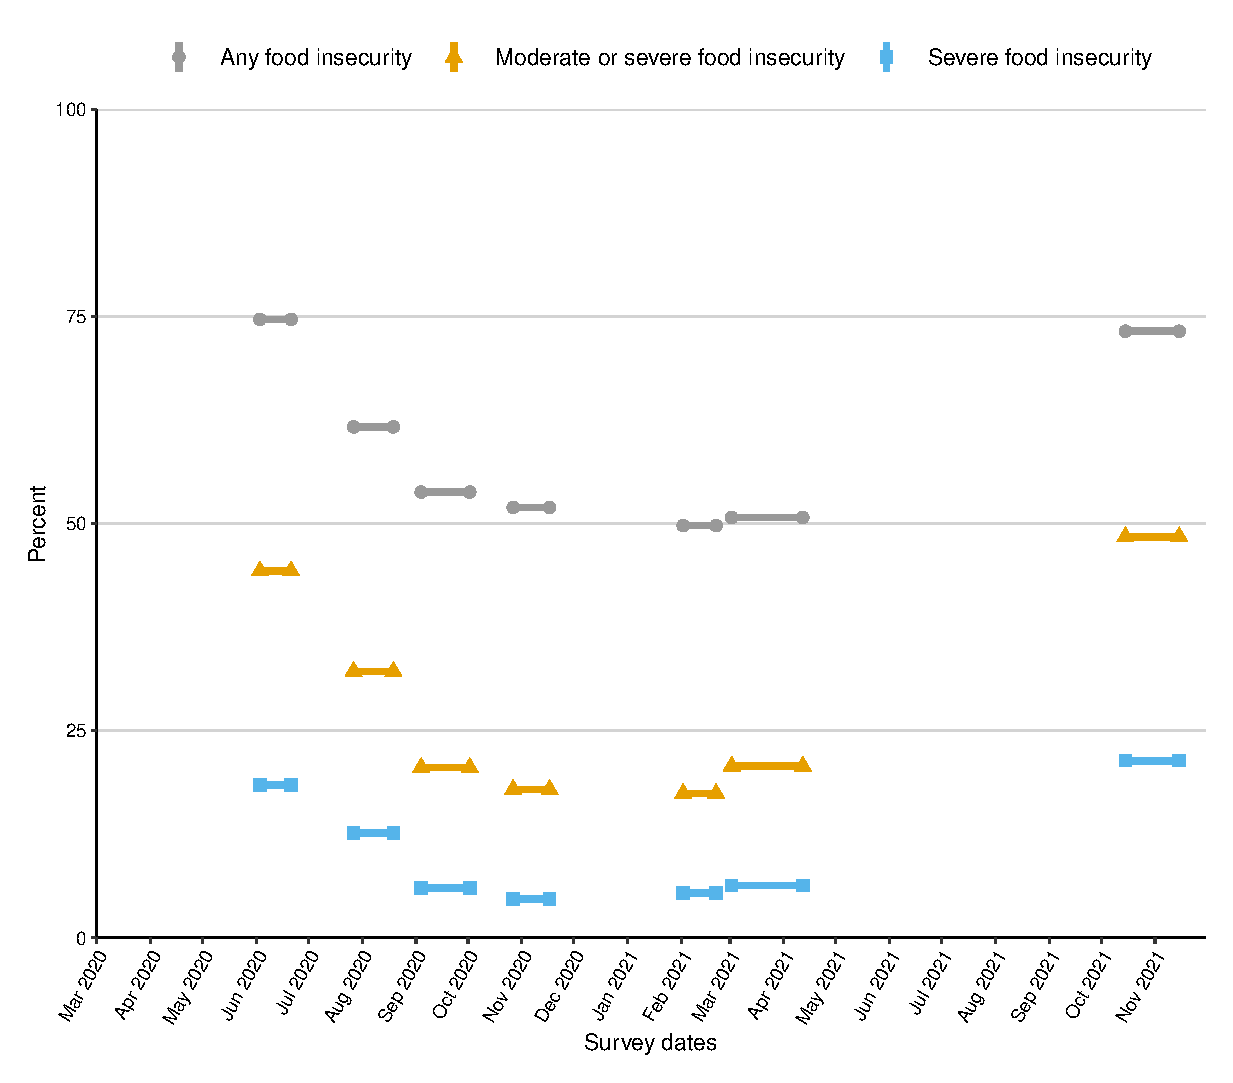
\includegraphics[width=\linewidth, keepaspectratio]{./eps/fig_01.eps}
\end{center}
\figuresource{Authors’ analysis based on data from the Uganda High-Frequency Phone Survey, Rounds 1-7.} 
\figurenote{Severe lockdowns shaded in grey. Lines cover start date to end date of each survey round.}
\end{figure}

To achieve this, we compare periods after severe lockdowns with other
periods during COVID-19 where the restrictions were less severe. The
initial lockdown was initiated well before any substantial spread of
COVID-19, which allows us to isolate the effect of the first severe
lockdown from the effect of the spread of the disease itself. The second
lockdown illustrates the effects of a second aggregate shock, just as
the economy was recovering.

Understanding how lockdowns impacted food insecurity and how households
responded to them is relevant for three reasons. First, it provides us
with a way to learn about the effects of aggregate/covariate shocks and
how households respond to them. Second, households are still in the
process of recovering from these shocks and likely will be for a
substantial period, and this type of analysis can serve as a starting
point for estimating the costs of the lockdowns. Last but not least,
understanding the cost and benefits of lockdowns is an important input
into planning for future pandemics and the appropriate policy response
to them \citep{World-Health-Organization2022}. The importance of this is
illustrated by the September 2022 Ebola outbreak in Uganda, which
resulted in a two-month lockdown with travel restrictions in the
affected districts
\citep{Makerere-University-School-of-Statistics-and-Planning2023}.\footnote{Work
  on the effects of Ebola outbreaks shows significant, and often
  long-lasting, impacts on food security and livelihoods in the affected
  communities, across Liberia, Sierra Leone, and Uganda, although
  separating out effects of the disease and the lockdowns is difficult
  \citep{Langlay2014, Himelein2015, Gatiso2018, Djomaleu2022, Makerere-University-School-of-Statistics-and-Planning2023}.}

Assessments in low- and lower-middle-income countries have found a mixed
impact of lockdowns on food insecurity when identifying the effect
through spatial or temporal variation in lockdowns.\footnote{A large
  number of studies provide cross-sectional evidence on food insecurity
  prevalence during COVID-19 and how it varies with household
  characteristics but do not attempt to identify the effects of
  lockdowns
  \citep{Ceballos2020, Ceballos2021, Dasgupta2021, Egger2022, Gaitan-Rossi2021, Giacoman2021, Harris2020, Jaacks2021, Kansiime2021, Kesar2021, Kundu2021, Lee2022}.
  Similarly, for income, employment, agricultural production, and
  savings
  \citep{Balde2021, Deshpande2020, Egger2022, Harris2020, Jaacks2021, Kang2021, Kesar2021, Komin2021, Ronkko2022, Siwach2023}.
  Even for countries with limited lockdowns and few COVID-19 cases, the
  associated price shocks lead to worsening food security
  \citep{Alam2024}.} The Bangladeshi lockdown exacerbated food
insecurity for urban low-income groups and in rural areas
\citep{Hamadani2020, Ruszczyk2021}. Households with mothers with very
young children in Uttar Pradesh saw a sharp increase in food insecurity
compared to pre-COVID-19 \citep{Nguyen2021a}. In Nigeria, higher
COVID-19 case rates and lockdown measures increased food insecurity,
particularly for households relying on non-farm businesses and those in
remote and conflicted-affected zones \citep{Amare2021}. Similarly, in 14
refugee-hosting settlements and the associated host community in Uganda,
lockdowns were associated with increased food insecurity and worsening
diet quality, with refugees being more affected than hosts
\citep{Squarcina2022}. However, in Ethiopia, Kenya, Liberia, and Malawi,
there was no evidence of increased food insecurity with lockdowns
\citep{Janssens2021, Aggarwal2022, Hirvonen2021}.\footnote{In the
  middle-income countries of Chile, Guatemala, and Peru, lockdowns were
  all associated with increased food insecurity
  \citep{Ceballos2021a, Curi-Quinto2021, Giacoman2021}.}

There is more consensus on the negative effects on income and employment
during the pandemic \citep{Schotte2023, Mahmud2023}. This reduced income
in the initial phases of the pandemic was associated with increased food
insecurity in Uganda, particularly in rural areas \citep{Agamile2022}.
Furthermore, there is evidence that households tried to cope with the
pandemic and lockdowns and through behavior changes, such as reducing
non-food expenditure, drawing down savings, leaving savings and loan
groups, increased borrowing, and selling assets
\citep{Ceballos2020, Kansiime2021, Mahmud2023, Ronkko2022, Ruszczyk2021}.
In addition, remittances declined, and there were insufficient or
delayed government support to help households cope with the shock
\citep{Ceballos2021, Curi-Quinto2021, Suresh2022}.

This study contributes to two strands of the literature. First, it
contributes to the literature on understanding the impacts of the
lockdowns themselves. Given the mixed findings and the limitations in
data in the prior literature, we use household fixed-effects models on
country-wide panel data to estimate short- and medium-run effects of
lockdowns, with the goal of understanding the persistence of the impact
of lockdowns in the months following their lifting.

Second, it contributes to the small but growing body of research on the
effects of aggregate shocks and how households cope with these shocks,
which has mostly focused on financial shocks and natural disasters
\citep{Del-Ninno2003, Fallon2002, Glewwe1998, Hallegatte2020, McKenzie2003, Skoufias2003, Thomas2007}.
First, we examine a repeated systemic shock, of which the first instance
was almost entirely unanticipated. Second, we directly analyze four
broad categories of coping mechanisms that households may use to
mitigate the effects of these shocks. The categories are changes in
labor market participation, diversification of income sources, transfers
and remittances, and changes in household structure through migration
\citep{Foster2002, Jayachandran2006, Kochar1999, McKenzie2003, Morduch1995, Townsend1994, Yang2007}.
Our paper complements recent work showing that rural households in
Uganda---especially non-farm business owners---experienced significant
asset decline and increased likelihood of net borrowing, presumably as a
coping mechanism after the first lockdown \citep{Mahmud2023}.

Compared to the prior literature, three things set our paper apart.
First, it uses a nationwide representative longitudinal survey. This is
in contrast to much of the prior research, which is based on either very
small samples
\citep{Ruszczyk2021, Squarcina2022, Hirvonen2021, Nguyen2021a} or only
rural areas \citep{Janssens2021, Aggarwal2022}. Second, the data covers
almost the entire pandemic, so we can observe the changes in food
insecurity and household responses over time and through multiple
lockdowns.\footnote{The other study using nationwide representative data
  only cover one survey round, April-May 2020, although more are planned
  \citep{Amare2021}.} Third, with very few COVID-19 cases in Uganda,
especially for the first lockdown, we can separate the effects of
COVID-19 from lockdown effects. However, there are at least three
potential drawbacks to our approach. First, phone surveys, as we use
here, provide less detailed data about household members and may suffer
from selection bias. Second, in contrast to, for example,
\citet{Amare2021}, there is limited pre-COVID-19 information on the
households. Third, there was no spatial variation in the lockdowns
decreed by the government, opposite of, for example, Nigeria or India.
Hence, identification is based on comparing periods with varying degrees
of restrictions, and our estimates are, therefore, likely lower-bound
estimates.

Food insecurity significantly increased during the lockdowns. The point
estimates are significant, with an increase of almost 25 percentage
points for any food insecurity during the first lockdown compared to the
period with no lockdowns. Even more concerning, moderate to severe and
severe food insecurity is more than 20 percentage points and almost ten
percentage points higher relative to when there are fewer
lockdown-related restrictions.

Lockdowns also have a substantial medium-term impact, with any food
insecurity about ten percentage points higher two to three months after
the first lockdown was lifted. The medium-term impact was even higher
following the second lockdown, with an approximately 20 percentage
points increase three months after the second lockdown had been lifted.
The differences in the medium-run impact between the two lockdowns
suggest that the lower-than-normal rainfall during July through October
of 2021 compounded the negative effect of the lockdown.

To understand the mechanisms behind the significant impact on food
insecurity, we examine the effect on labor market outcomes and find
substantial decreases across all income types, such as wage income,
agricultural income, non-farm business income, and income from assets
owned. There were also substantial decreases in the likelihood of
engaging in market work during the lockdowns. Households in the
agricultural sector saw lower increases in food insecurity than
non-agricultural households, especially for severe food insecurity,
during the first severe lockdown. This is consistent with agricultural
households being able to work even during lockdowns and have access to
foods produced at home.

Furthermore, households attempted to cope with the lockdown by switching
to agricultural work, as shown by a significant increase in the
likelihood of working in agriculture after the first lockdown. However,
likely because the concurrent rainfall shortfall made agriculture less
attractive as a coping mechanism, there was no further movement to
agriculture after the second lockdown.

Traditional sources of support, such as remittance from abroad or
assistance from family members within the country, non-family
individuals, and development organizations, were all either flat or
decreased during the lockdowns. This suggests that the worldwide
macroeconomic shock from COVID-19 affected everyone's ability to
transfer resources to needy relatives or friends. This failure of the
standard coping mechanisms is likely a significant factor in explaining
lockdowns' substantial effect on food insecurity.

\section{Data}\label{data}

Household and individual data come from the Uganda High-Frequency
Phone Survey on COVID-19 (UHFS), conducted by the Uganda Bureau of
Statistics in collaboration with the World Bank. The survey was
conducted in seven waves, with four waves in 2020 (June, August,
September, and October) and three in 2021 (February, March, and
October). The goal was to understand the economic and social impacts of
the COVID-19 pandemic by collecting high-frequency data on individuals
and households \citep{Uganda-Bureau-of-Statistics2022}. To this end, the
survey asked detailed questions on food insecurity, employment, income,
outside assistance, and agricultural practices.

The UHFS sample is a subset of the 3,098 households interviewed in the
8th wave of the Uganda National Panel Survey in 2019/20 (UNPS 2019/20).
In UNPS 2019/20, respondents were asked to provide a phone number where
they could be reached, either their own or that of a friend or neighbor.
Originally, the goal was to ensure households could be reached in case
they moved, but with the COVID-19 lockdowns, the phone numbers became
the basis for surveying households. Of the 2,386 households that
provided a phone number, 2,225 were successfully interviewed for Round 1
of the UHFS. The head of the household was typically the respondent. If
the household head was not present, another member of the household over
the age of 15 could respond to the survey.

A concern with phone surveys is that households with access to phones
are fundamentally different from households without access to phones. It
is, for example, possible that phone surveys have a higher likelihood of
reaching wealthier households, who typically have better access to
phones, than poorer households. This would bias our results. To avoid
any biases to the extent possible, we use the UHFS-provided survey
weights to ensure that the data is nationally representative
\citep{Uganda-Bureau-of-Statistics2022}.

Over the seven rounds, the cumulative attrition rate was 15.8 percent of
the originally surveyed households from Round 1, with 1,873 households
from the baseline interviewed in Round 7 (October 2021). However,
replacement households were added to the sample following the first
round. This brings our total sample size to 2,334 households. The number
of original households that remained in each round together with the
number of new households added in the follow-up rounds and the total
number of households per round are presented in Appendix Table
\ref{tab:surveys}.

\subsection{Food Insecurity Measurement}\label{food-insecurity-measurement}

The surveys measured food insecurity based on the Food Insecurity
Experience Scale (FIES) developed by the FAO \citep{FAO2016}. FIES uses
eight questions with dichotomous (yes/no) responses to capture different
aspects of food insecurity. The questions are whether, during the last
30 days, there was a time when any adult in the household experienced
the following because of lack of money or other resources: (i) were
worried about not having enough food to eat; (ii) were unable to eat
healthy and nutritious/preferred foods; (iii) ate only a few kinds of
foods; (iv) had to skip a meal; (v) ate less than you thought you
should; (vi) ran out of food; (vii) were hungry, but did not eat; and
(viii) went without eating for a whole day.

Following the prior literature, three food insecurity measure based on
the sum of the eight food insecurity questions are calculated: any,
moderate or severe, and severe food insecurity
\citep{Kansiime2021, Wambogo2018, FAO2016}. ``Any'' corresponds to
having answered yes to any of the questions, ``moderate or severe'' to
having answered yes to four or more, and ``severe'' if answered yes to
seven or eight questions \citep{FAO2015, FAO2016}.\footnote{Results for
  the estimations below using each individual question as the dependent
  variable are available upon request.}

Although the sample for the UHFS is based on the UNPS 2019/20, there is,
unfortunately, no direct way to compare food insecurity across the
surveys. First, the UNPS 2019/20 questions have a broader scope, which
includes situations such as insecurity in reaching the market, the
absence of food in the market, and floods, rather than the lack of money
or other resources in the FIES questions. Second, the only food
security-related question in UNPS 2019/20 asked whether there has been a
situation in the last 12 months when there was not enough food to feed
the household, with a follow-up question about which months this
happened in and an open-ended question about why it happened. These do
not match up with any of the individual FIES questions or the cumulative
food insecurity measures that we use. Finally, the UHFS questionnaire
asks about the respondent and other adults in the household, rather than
the entire household as in UNPS 2019/20. As long as children are kept
fed even in times of food insecurity, this does not in itself prevent
comparison, but it is possible that food goes to the most productive
members of the household in order to preserve his or her productivity
\citep{Pitt1990}.\footnote{A minor point of difference is that the UNPS
  2019/20 asks about individual months, whereas the UHFS asks about the
  last 30 days before the interview, which, depending on when the survey
  took place, does not line up with the month-centric question of the
  UNPS 2019/20.}

\section{Lockdown Context and Enforcement}\label{lockdown-context-and-enforcement}

On March 18, 2020, the Ugandan government began imposing restrictions,
including travel restrictions and cancellation of public gatherings,
such as religious services, weddings, and music events
\citep{Uganda-Bureau-of-Statistics2022}. On March 20, schools were
closed, and a total lockdown was imposed on March 30 with a nationwide
curfew from 7 pm to 6:30 am, banning of public transportation, strict
regulations on the movement of vehicles, and closure of all
non-essential businesses, which extended till the end of May
\citep{Alfonsi2021, Margini2020}.

Lockdowns were eased at the beginning of June 2020 with the resumption
of public transportation and the opening of businesses
\citep{Guloba2021, Monitor2020, Schwartz2021, Wagner2022}. Most small
and medium businesses were back open by July-August 2020
\citep{Alfonsi2021}. International travel restrictions remained until
the end of September, when land borders reopened, and international
flights resumed \citep{Guloba2021}.

In response to the increasing number of COVID-19 infections in 2021, the
government of Uganda imposed a second severe lockdown from mid-June 2021
\citep{Atamanov2022, Athumani2021}. This second lockdown was partly
eased by the end of July 2021 \citep{Biryabarema2021}.

To show the strictness of the lockdowns imposed, we employ a modified
version of the lockdown stringency index developed at the Blavatnik
School of Government, University of Oxford (Hale et al., 2021). The
original index is a daily composite measure of how strict the lockdowns
were based on nine indicators, including school closures, workplace
closures, and travel bans, rescaled to a value from 0 to 100, where 100
is the strictest response. As some of the restrictions in the original
index, such as school closure and international entry restrictions, are
likely to have minimal immediate impacts on food insecurity, we
recalculate the index using workplace closings, limits on public
transport, stay-at-home requirements, and any restrictions on internal
movement.

The stringency index cannot capture the extent to which the lockdown
policies were enforced or adhered to, and we, therefore, also use Google
Mobility data on the percentage change in the number of visitors to
retail and recreation locations relative to the pre-COVID-19 behavior
\citep{Google2022}. We use this measure because it captures the closures
of shops and has better regional coverage than most other mobility
measures.\footnote{Mobility information for the five other locations
  types, the percentage change in the number of visitors to workplaces
  to groceries or pharmacies, to transit stations, to parks, and the
  percentage change in the time spent at residential locations are shown
  in Figures S1.1 through S1.5  in the supplementary online appendix, available 
  with this article at The World Bank Economic Review website.
  The visits to workplaces measure also has good regional coverage but it is unclear
  how relevant this is given that the majority of people in Uganda work
  in agriculture.} Each day of the week is scaled relative to a
``baseline day,'' which is the median value from the five weeks, January
3 -- February 6, 2020.

\begin{figure}
\caption{Revised stringency index, visits to retail and recreation
locations, daily new COVID-19 cases per 100,000 persons and new deaths
per 100,000, and data collection window for each UHFS survey
round}\label{fig:combined}
\begin{center}
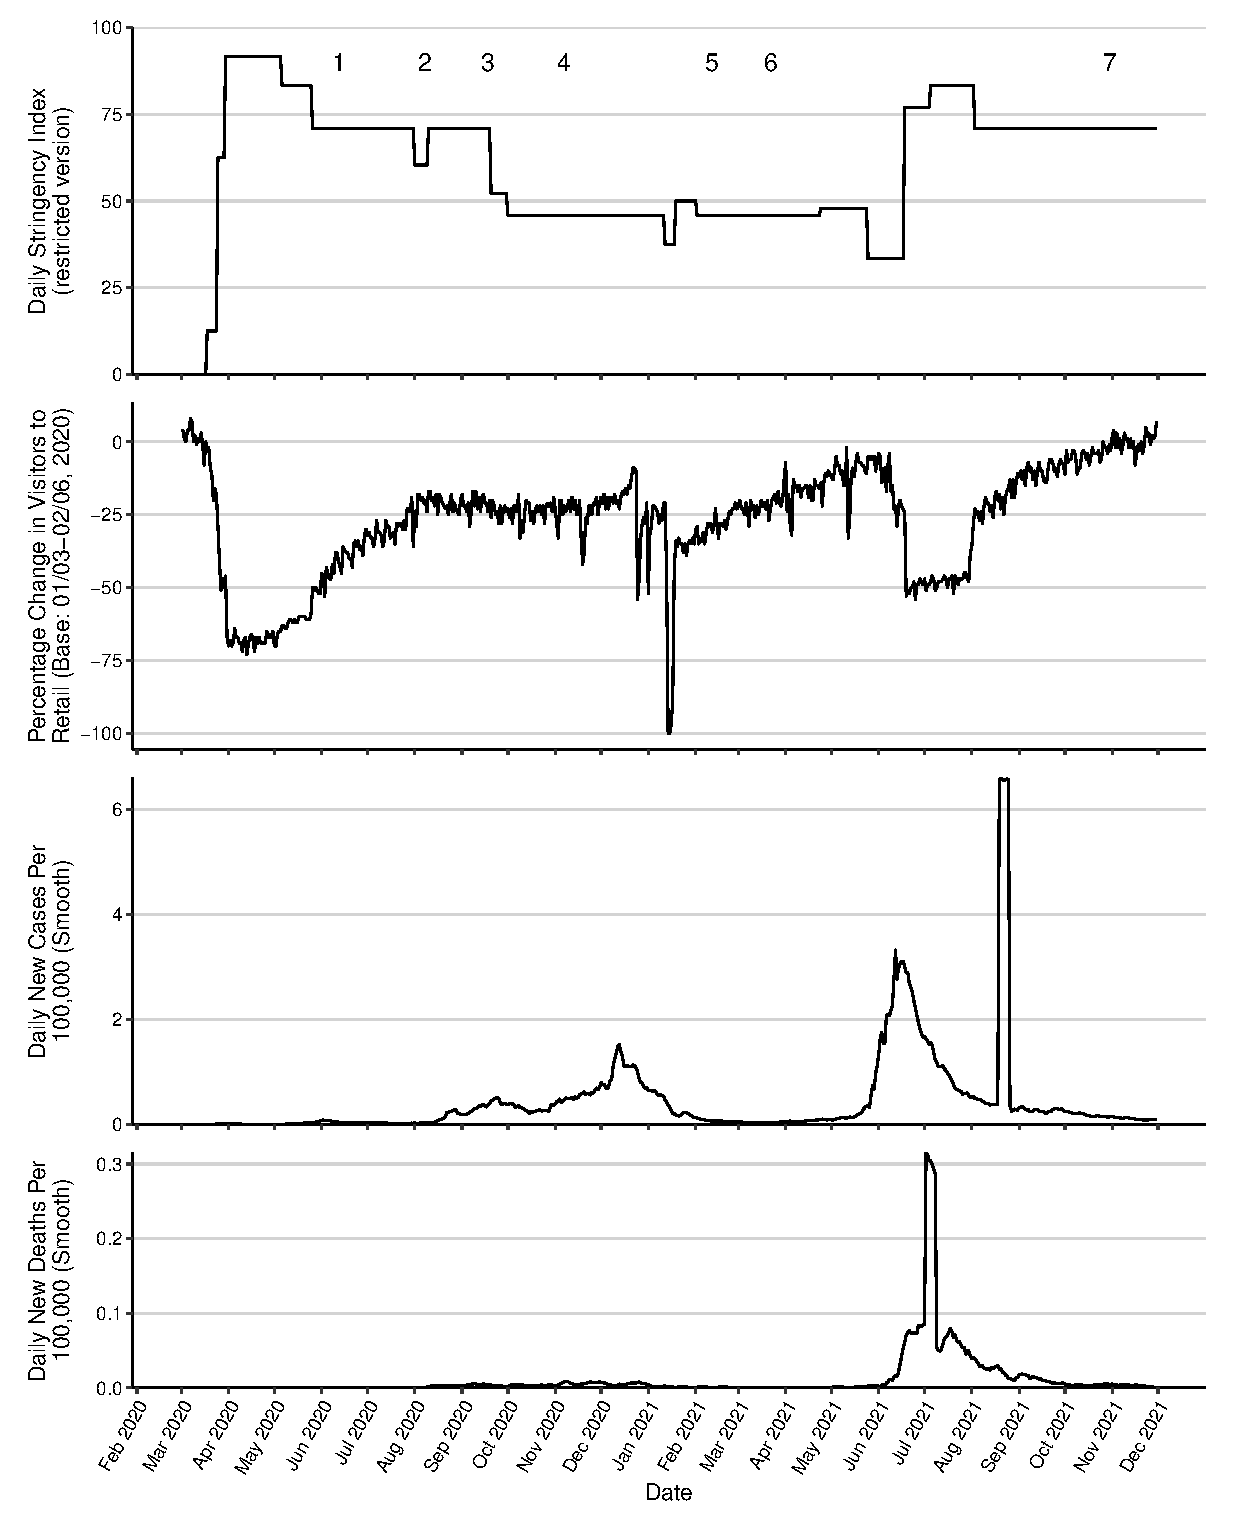
\includegraphics[width=\linewidth, keepaspectratio]{./eps/fig_02.eps}
\end{center}
\figuresource{Authors' analyses based on the following: 
    for the Daily Stringency Index, the lockdown stringency index developed 
    at the Blavatnik School of Government, University of Oxford;  
    for the Percentage Change in Visitors to Retail, data from Google Mobility;
    for the Daily New Cases and Daily New Deaths, data from Our World in Data;
    and the survey dates from Uganda High-Frequency Phone Survey.} 
\figurenote{Grey shaded areas indicate start date to end date for each of the seven survey rounds.}
\end{figure}

Figure \ref{fig:combined} shows the daily stringency index, the daily
Google Mobility measure, the 7-day average number of new COVID-19 cases
and deaths per 100,000 persons, and the data collection window for each
of the UHFS rounds in shaded grey. The number of COVID-19 cases and
deaths comes from ``Our World in Data.''\footnote{The advantage of using
  ``Our World in Data'' is that it collects available COVID-19 data from
  many sources. The data are available
  at \url{https://covid.ourworldindata.org/data/owid-covid-data.csv},
  and a complete listing of underlying sources is
  at \url{https://github.com/owid/COVID-19-data/tree/master/public/data/owid-covid-codebook.csv}.}

The strictest restrictions are just before Round 1, where there is an
almost complete lockdown. According to the stringency measure, the
second lockdown---in June and July 2021---was nearly as strict as the
first. Furthermore, the four months after each lockdown show similar
stringency levels.

That the most severe lockdown policies were enforced is evident from the
substantial decreases in visits to retail from April through June 2020
and June through August 2021, with close to 75\% and 50\% decreases,
respectively. Despite the remaining restrictions during the second and
third rounds, the number of visits to retail locations slowly improved,
stabilizing at around 25\% below ``normal'' during the 4th through 6th
survey rounds. Only around May/June 2021 had retail visits returned to
almost the baseline level.

Outside of the severe lockdown periods, the time spent at home remained
relatively stable with three notable exceptions. The two most innocuous
are the closures around the Christmas and New Year's celebrations. The
third is the 2021 general election, which took place on 14 January. All
shops were closed on the day of the election, and nobody appeared to
have gone to any retail location immediately following the election.
Although the election was preceded by widespread violence and internet
shutdowns immediately around the time of the election, the reduction in
visits to retail and recreation locations appeared to have been
relatively short-lived.

The number of confirmed infections and deaths from COVID-19 remained low
in Uganda until halfway through 2021. For context, even with the spike
in cases in 2021, Uganda's cumulative number of cases per 100,000 at the
end of 2021 was only 306.9 compared with 16,294.5 in the US.
Furthermore, as in many other developing countries, the number of
COVID-19 deaths was low. Even with the increase in cases and deaths by
the end of 2021, Uganda had only 7.2 deaths per 100,000 persons, while,
for comparison, the US had 245.1 deaths per 100,000 persons.

On top of lockdowns and COVID-19, the later part of 2021 saw a
below-normal rainfall during the rainy season across the country. The
three-month 3-month rainfall was 75\% of normal when averaged across all
measurement stations, and all stations showed a below-normal three-month
rainfall in August 2021.\footnote{Calculations based on data available
  at
  \href{https://data.humdata.org/dataset/uga-rainfall-subnational}{https://data.humdata.org/dataset/uga-rainfall-subnational}.}

\section{Estimation Strategy}\label{estimation-strategy}

To examine the effects of COVID-19 lockdowns, we use household
fixed-effects models on a nationally representative longitudinal
household data set, relying on the changes over time in
government-imposed lockdowns to identify the effect.

Our main specification regresses outcomes, \(Y\), on a set of variables
using a linear fixed-effects model:\footnote{A linear model has two
  advantages over non-linear models, such as conditional logit, and has
  often been used in recent studies
  \citep{Alam2020, Alam2018, Charles2008}. First, coefficients are
  easier to interpret. Second, a linear model allows a more
  straightforward comparison of coefficients across regression where
  some dependent variables are binary and some non-binary. Robustness
  checks, available upon request, show that conditional logit models
  lead to similar results.}

\[
Y_{i,t} =  \sum_{t=1}^7 \beta_t 1[Round = t]  + \gamma Cases_{t} 
+ \omega_i + \epsilon_{i,t}, 
\]

where \(i\) denote household and \(t\) survey rounds. All standard
errors control for clustering at the primary sample unit level.

We use survey indicator variables to capture the variation over time.
The first survey round took place between 9 and 27 days after the end of
the first severe lockdown and, therefore, can be thought of as capturing
the short-run effect of the first lockdown. The second survey took place
63 to 86 days after the first lockdown ended and the seventh survey took
place 74 to 105 days (with the majority within 87 days) after the second
lockdown ended. These we refer to as medium-term. The third, fourth,
fifth, and sixth survey rounds took place 112--130, 155--176, 253--272,
and 281--322 days after the first severe lockdown. We use the fourth
survey round as the excluded round because it is the survey round
furthest from both lockdowns and before any substantial number of
COVID-19 cases, and before the general election begins in earnest.

In addition to government-imposed lockdowns, individuals may be ill,
decide to self-isolate, or take other steps to avoid contact with others
if they perceive a high risk of contracting COVID-19, which may increase
food insecurity. To capture the severity of the COVID-19 situation, the
\(Cases\) variable measures the number of new COVID-19 cases per 100,000
persons in the 30 days before the household's survey date.
Unfortunately, there is no information available on the number of
COVID-19 cases at a more granular level than the country level.

Although we do not include any household-level variables in the model,
there are still three advantages to using a fixed effects model. First,
the fixed effects estimates are more conservative than pooled OLS in the
sense that fixed effects models have a lower likelihood of type I errors
and potential attenuation bias toward zero with classical measurement
error. Second, fixed effects models are more robust to measurement
errors that vary systematically across individuals than pooled OLS. For
certain food insecurity questions, such as, for example, those that
refer to healthy food, the diversity of foods available, and eating less
than desired, there may be individual-specific threshold levels. The
within-household fixed effects model reduces the potential bias from
this type of measurement error because it relies only on
within-household variation. Finally, the household fixed-effects,
\(\omega_i\), control for time-invariant characteristics associated with
the individual/household, such as gender, race and religion, constant
preferences, household characteristics, and area characteristics,
thereby absorbing the variability in the dependent variable due to
household-specific characteristics and reducing the residual variance.
This reduction in residual variance can lead to more precise estimates.
For some estimations, we use individual-level dependent variables, like
employment. In these cases, the models are individual fixed-effects
models, as the same individual from the household is followed over the
rounds.

In summary, we identify the impact of Uganda's lockdowns by comparing
periods with more or less severe lockdowns, while the individual survey
round indicators capture other potential factors that might impact food
insecurity, such as seasonality and the unrest in connection with the
2021 general elections. Especially the first lockdown is of interest
because it came at a time when there were close to no COVID-19 cases,
and, in fact, there was no substantial spread of COVID-19 until well
after the first severe lockdown ended. Hence, we can identify the effect
of the lockdown as opposed to the aggregate effect of the lockdowns and
the spread of the disease combined.

To ensure that we are not capturing other changes, we also examine the
potential role of seasonality in the results. Finally, there were no
official variations in lockdown policies or enforcement across different
areas, and we, therefore, cannot rely on spatial variation for
identification. Instead, we examine differences in mobility patterns and
food insecurity across regions.

\section{Did Lockdowns Increase Food
Insecurity?}\label{did-lockdowns-increase-food-insecurity}

\begin{figure}
\caption{Estimated changes in food insecurity with 95\% confidence
intervals by survey round relative to Round 4, controlling for number of
COVID-19 cases and household fixed
effects}\label{fig:food_insecurity_survey}
\begin{center}
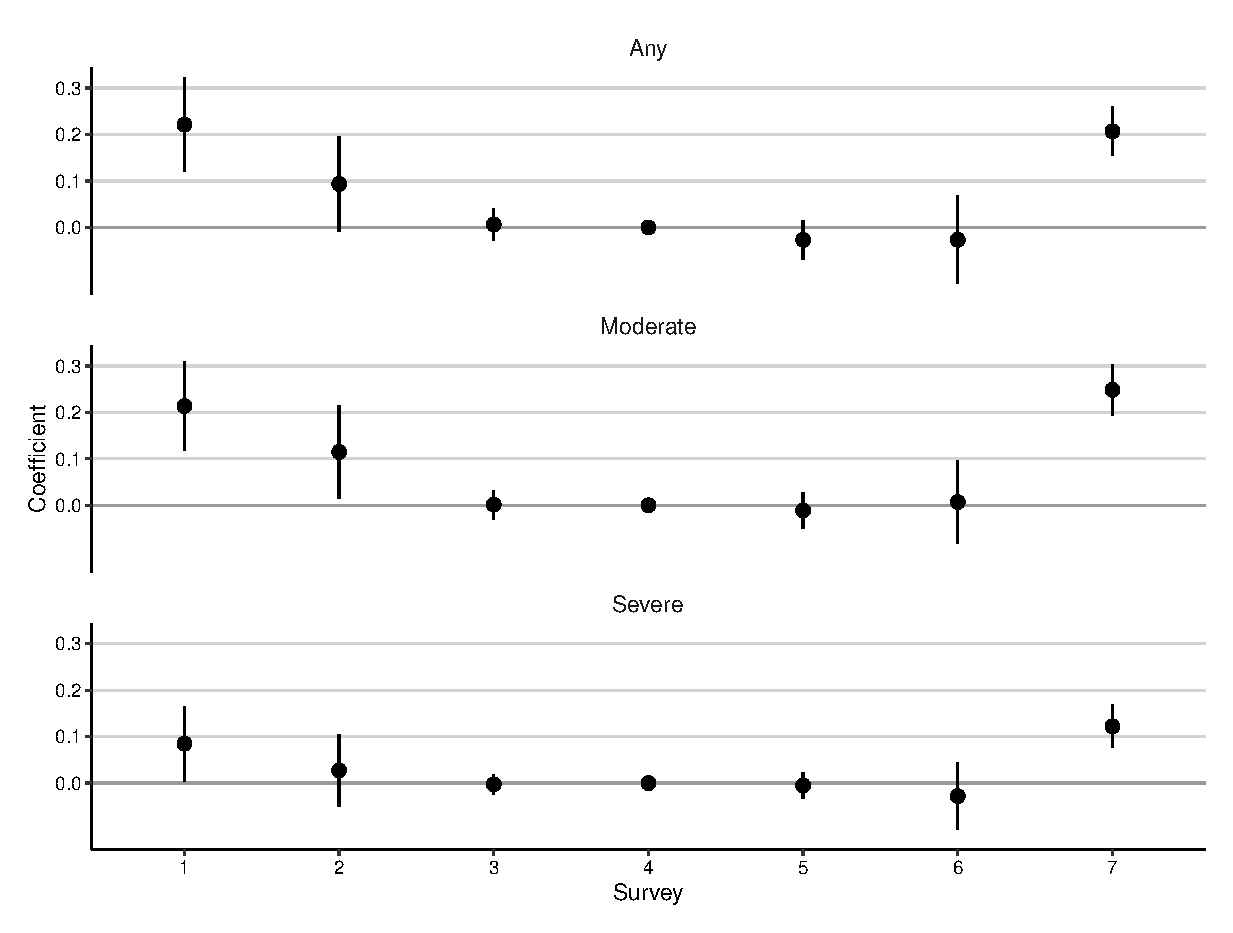
\includegraphics[width=\linewidth, keepaspectratio]{./eps/fig_03.eps}
\end{center}
\figuresource{Authors’ analysis based on data from the Uganda High-Frequency Phone Survey, Rounds 1-7.} 
\figurenote{Household fixed effects estimates relative to Round 4.}
\end{figure}

Figure \ref{fig:food_insecurity_survey} shows the estimated changes in the
three food insecurity measures by survey round, relative to survey Round
4, together with the 95\% confidence intervals for a linear model with
household fixed effects.\footnote{The full tables for this and all
  following results presented as tables are available upon request.}
Overall, COVID-19 lockdowns appear to be associated with substantial
increases in all levels of food insecurity.

Approximately a month after the end of the first severe lockdown, the
proportion of households that report any or moderate to severe food
insecurity is more than 20 percentage points higher than in Round 4, an
effect that is statistically significant. Severe food insecurity in
Round 1 is just below 10 percentage points higher than in Round 4 and
also statistically significantly different from Round 4.

About three months after the end of the first severe lockdown, any and
moderate to severe food insecurity levels are still statistically
significantly higher than in Round 4 at approximately 10 percentage
points. Severe food insecurity is also increased but not statistically
significantly so.

Between six and eleven months (Rounds 3 through 6), there is little
discernable difference in the levels of food insecurity, and we cannot
reject that they all have the same levels.

The final round, Round 7, took place 2.5 to 3.5 months after the end of
the second major lockdown, but in relation to Round 4, the levels of
food insecurity are closer to those of Round 1. Any and moderate to
severe food insecurity are both more than 20 percentage points higher
than in Round 4, while severe food insecurity is more than 10 percentage
points higher; all three are strongly statistically significant. These
medium-term effects are close to the short-run effect of the first
severe lockdown.

How do these results compare to those in the prior literature? As
discussed in the Introduction, among the studies that try to provide
causal evidence based on panel data, most do not find an impact on food
insecurity. The exception is for Nigeria, where there was a 39
percentage-point increase in the likelihood of skipping a meal and an 11
percentage-point increase in going without eating a whole day. However,
two factors make comparison difficult: the results are based on
comparison with pre-COVID-19 data rather than within the COVID-19
period, and do not use the Food Insecurity Experience Scale (FIES)
\citep{Amare2021}.

Two studies are of particular interest here as they use data from Uganda
\citep{Kansiime2021, Agamile2022}. \citet{Kansiime2021} find that food
insecurity increased by 44, 30, and 7 percentage points for any,
moderate, and severe levels, respectively, five weeks into the first
lockdown compared to ``normal.'' Howevever, these results are based on a
non-representative sample of 129 respondents using a Google form
distributed via social media. \citet{Agamile2022} uses a subset of the
same data as here, covering Rounds 1 through 5, and finds, for example,
that going without food the entire day is 4.8 percentage points higher
in Round 1 than in Round 5, and the likelihood of running out of food
8.9 percentage points higher. However, direct comparison is complex, and
not just because the outcomes are seven individual food security
questions rather than the FEIS. The goal of the analysis in
\citet{Agamile2022} is to examine the effects of income loss on food
security rather than the overall effect of the lockdowns, and the Round
indicators, therefore, capture the difference to the excluded Round 5,
conditional on the households' occupations, reductions in various income
sources, region dummies, and a set of household characteristics.
However, as shown below, most of these variables change in response to
the lockdowns, and the Round indicators are, therefore, not estimates of
the lockdown's effect. Furthermore, the estimation methods do not use
household fixed effects or control for the number of COVID-19 cases.

\subsection{The Role of Seasonality}\label{the-role-of-seasonality}

Uganda has two lean seasons, one in April and May and another in
November and December \citep{FAO2022}. Hence, with the first survey
round fielded in June 2020, it is possible that part of what we capture
with the Round 1 indicator variable is the effect of the April/May lean
season on food security. To examine the role of seasonal variation, we
compare the changes in food insecurity measures with the closest
comparable from previous rounds of UNPS 2019/20 and estimate our main
model on alternative samples to show that seasonal variation is unlikely
to explain our results.

To examine whether seasonality in food security might be behind our
results, we first compare pre-COVID-19 information on food insecurity
with a subset of our measures. The UNPS 2015/16 and the UNPS 2019/20
both asked if the households had been faced with a situation when they
did not have enough food to feed the household in the last 12 months. If
yes, they were asked to list all months when this occurred. Although
this question does not directly correspond to any of the food insecurity
questions asked in the UHFS and the recall period is one year rather
than the 30 days for the UHFS, it is close to three of our questions:
ran out of food because of lack of money, went hungry but did not eat,
and went without eating for a whole day.

For the UNPS question, we combined all observations from 2015/16 and
2019/20 by month, and calculated the percentage who reported not having
enough food to feed the household. For the UHFS questions, we calculate
the percentages of food insecure by interview month.
Figure \ref{fig:seasonality} shows the food insecurity percentages with
the UNPS question shown in black for comparison. Despite FAO listing
April/May and November/December as the lean periods, the UNPS data show
that April, May, and June were the three months with the highest
proportion of food insecurity, while November and December were the
months with the lowest proportion.\footnote{This pattern holds for both
  UNPS 2015/16 and UNPS 2019/20. The results for the individual surveys
  are available upon request. UNPS 2018/19 shows the same questions in
  the questionnaire, but the responses are not available in the data.}

\begin{figure}
\caption{Projected seasonality in food insecurity from UNPS and observed
food insecurity for three UHFS outcomes}\label{fig:seasonality}
\begin{center}
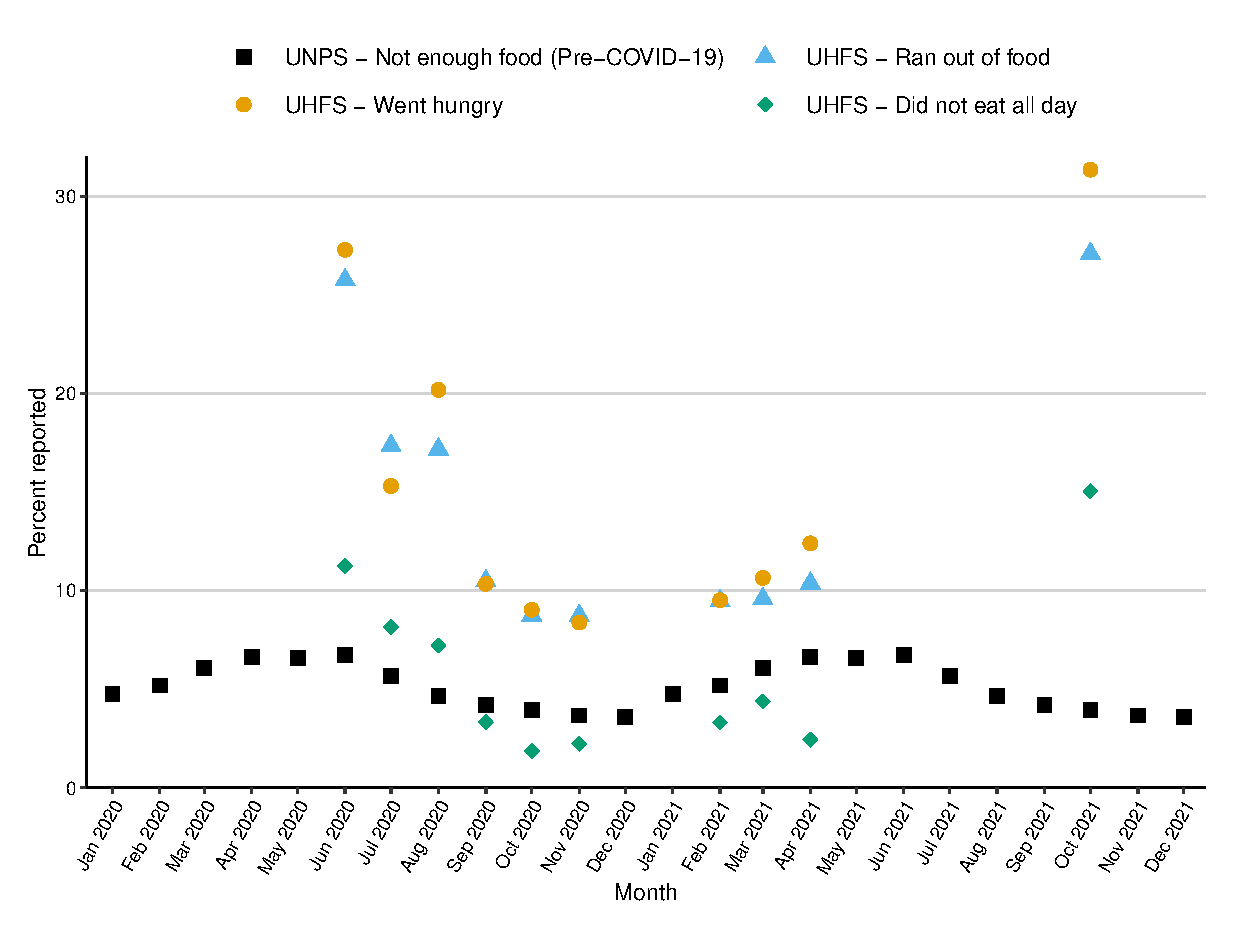
\includegraphics[width=\linewidth, keepaspectratio]{./eps/fig_04.eps}
\end{center}
\figuresource{Authors' analysis based on data from the 2015/16 and 
    2019/20 Uganda National Panel Survey (UNPS)  and data from the 
    Uganda High-Frequency Phone Survey (UHFS), Rounds 1-7.
} 
\figurenote{For the UNPS question, all observations from 2015/16 and 2019/20 
    are combined by month, and the percentage who reported not having enough 
    food to feed the household in each month calculated. 
    For the UHFS questions, the percentages of food insecure are calculated by 
    interview month.
}
\end{figure}


All three UHFS questions follow the same general pattern as the UNPS
question outside the lockdown periods, September 2020 through April
2021, while the months following the lockdowns are clearly elevated.
Although it is possible that these high values were the result of
seasonal variation, we consider it unlikely for two reasons. First,
there is no evidence of the same elevation for April 2021, which is also
in the lean season but nine months after the lockdown. Second, the
medium-term effects of the second lockdown show even worse medium-term
food insecurity outcomes despite being in a non-lean period.

Our second approach is to re-estimate our main models on three subsets
of the data. First, we make use of the fact that Round 6 took place
during the April/May lean season but was the round least affected by
lockdowns. Because Rounds 1 and 2 also took place during the lean
season, we estimate our main model using only information from Rounds 1,
2, and 6. The results are shown in the top panel of Figure S2.1. 
Compared to the main model, the short-run effects are slightly smaller 
and the medium effect larger.

Second, to show the robustness of the second lockdown medium-run
results, we make use of the fact that Rounds 4 and 7 were collected
during almost the same calendar month. The bottom panel of 
Figure S2.1 shows the results when we restrict
to those two rounds. The medium-run effect of the second lockdown for
this sample is smaller but still statistically significant in most
cases. Complicating this comparison is that the number of new COVID-19
cases was close to constant within each round and smaller during Round 7
than Round 4, resulting in potential multicollinearity and statistically
significant \emph{negative} effects of new cases on food insecurity for
some outcomes.

Finally, we expect urban households to be less affected by seasonality,
and Figure S2.2, therefore, shows the
results using only urban households across all rounds. The short- and
medium-run effects of the lockdowns are either the same or larger when
we restrict the sample to urban households. Hence, our results are
qualitatively the same, no matter how we account for seasonality.

\subsection{Regional Variation}\label{regional-variation}

All of the results above are national-level, which may obscure critical
regional variations in COVID-19 exposure and the degrees and effects of
lockdowns. This section, therefore, examines differences in the Google
Mobility measure and in food insecurity across the survey rounds for
each of the four regions in Uganda.

Uganda is divided into four regions, Central, Eastern, Northern, and
Western, which, although without direct administrative roles, are used
as units for statistical and planning purposes. The regions have
approximately the same population size, except for the Northern region,
which had 20\% of the population in the 2014 census.

The Central region is home to Kampala and the most urbanized, with the
four most populous urban centers in Uganda
\citep{Uganda-Bureau-of-Statistics2016}. Combined, these four urban
centers are home to one-third of the entire urban population of Uganda,
with almost 2.5 million people.\footnote{For comparison, the
  fifth-largest urban center, the Western region's Mbarara, had fewer
  than 200,000 people in 2014.} The region has a higher concentration of
service and industrial employment than the other regions and the lowest
poverty rates \citep{Ssewanyana2012}.

In contrast, employment in the other regions is predominantly
agricultural. The Eastern region is characterized by mixed farming,
including both crop cultivation and livestock, with a focus on cash
crops like coffee and tea. The Western region, rich in fertile soils and
rainfall, supports intensive agriculture, particularly dairy farming and
tea cultivation. The Northern region, historically affected by conflict,
has a more subsistence-oriented agricultural system, with lower levels
of productivity and a slower pace of urbanization, and consistently has
the highest poverty levels.

\begin{figure}
\caption{Regional distribution of percentage changes in the number of
visitors to retail and recreation locations}\label{fig:retail_regional}
\begin{center}
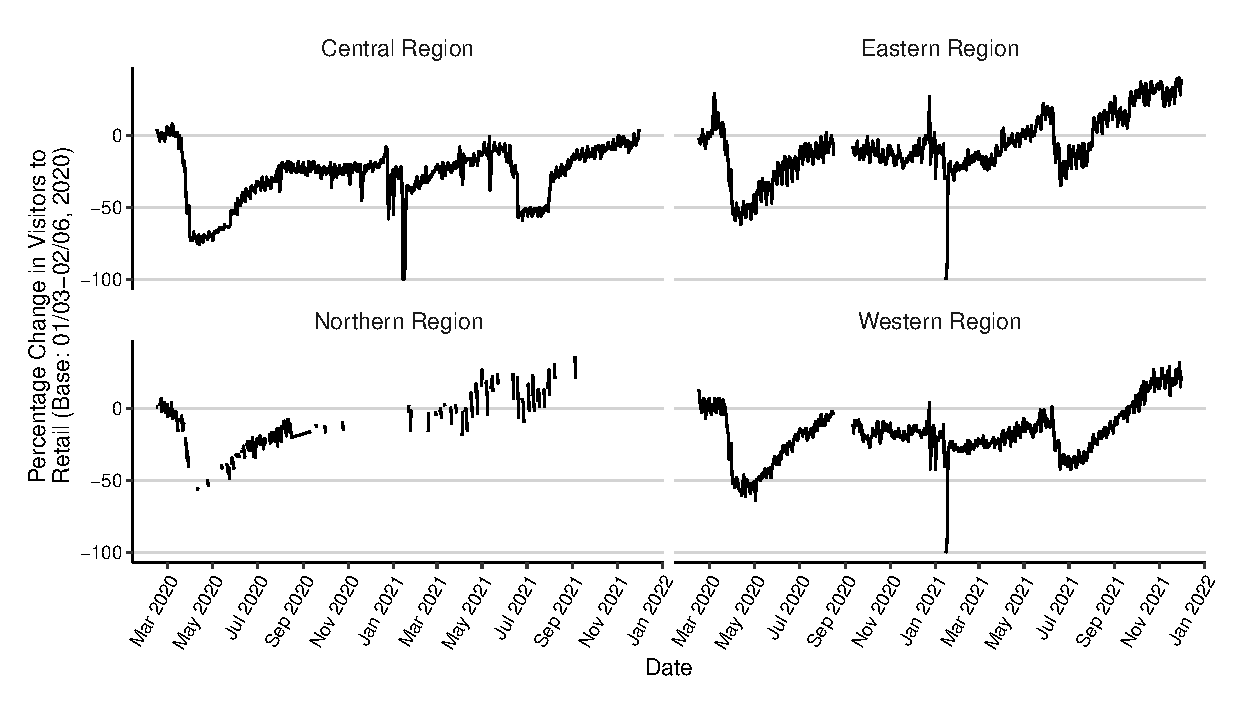
\includegraphics[width=\linewidth, keepaspectratio]{./eps/fig_05.eps}
\end{center}
\figuresource{Authors' analysis based on data from Google Mobility.} 
\figurenote{Missing are due to no data provided for those dates. Shaded areas represent the survey dates.}
\end{figure}

Figure \ref{fig:retail_regional} shows the percentage changes in visits to
retail and recreation locations by region, together with the survey
rounds.\footnote{Figures S3.2 through S3.6 show the
  percentage changes in the number of visitors to workplaces to
  groceries or pharmacies, to transit stations, to parks, and the
  percentage change in the time spent at residential locations. Although
  the workplace mobility data appear to have broader coverage we prefer
  the retail measure because of the predominately agricultural nature of
  work in the Eastern, Northern, and Western regions.} In all regions,
there is clear evidence of the scale of the first severe lockdown,
although the percentage change is larger in the Central region at about
75\%, compared with just over 50\% in the other three regions.

During the second severe lockdown, there is a smaller reduction in the
visits to retail locations than the first, but otherwise, it followed
close to the same regional pattern as the first lockdown. The Central
region showed the largest reduction at around 50\%. The Western and
Eastern regions both saw approximately 40\% reductions when compared to
the period immediately preceding the second main lockdown. The data for
the Northern region is spottier, but there is some evidence for a
reduction in visits compared to the period immediately before the second
lockdown.

These changes in visits to retail locations are consistent with more
heavily enforced lockdowns in urban than in rural areas. However, even
in the three more agricultural-focused regions, there are substantial
changes in mobility consistent with enforced lockdowns. For the second
lockdown, it is possible that part of the change in behavior comes from
self-isolation associated with the increasing number of COVID-19 cases,
although, unfortunately, no regional data is available to investigate
this possibility.\footnote{While we normally think of cities as having a
  higher communicable disease load than rural areas, this might not hold
  in the case of COVID-19. Rather, larger rural households may allow
  more people to be exposed to COVID-19 infections, especially if
  lockdowns are enforced in rural areas. Furthermore, people may be
  moving from urban to rural areas to ``escape'' increasing levels of
  COVID-19 infections, bringing COVID-19 with them to rural areas.}

Figure \ref{fig:food_insecurity_region} shows the results by level of food
insecurity and regions, where each region is treated as a separate
sample. The regional raw levels of food insecurity by round are shown in
Figure S3.1. Because we do not have information on regional COVID-19 cases, 
all models are estimated without COVID-19 cases variables.

\begin{figure}
\caption{Estimated changes in food insecurity with 95\% confidence
intervals for each region by survey round relative to Round 4,
controlling for household fixed
effects}\label{fig:food_insecurity_region}
\begin{center}
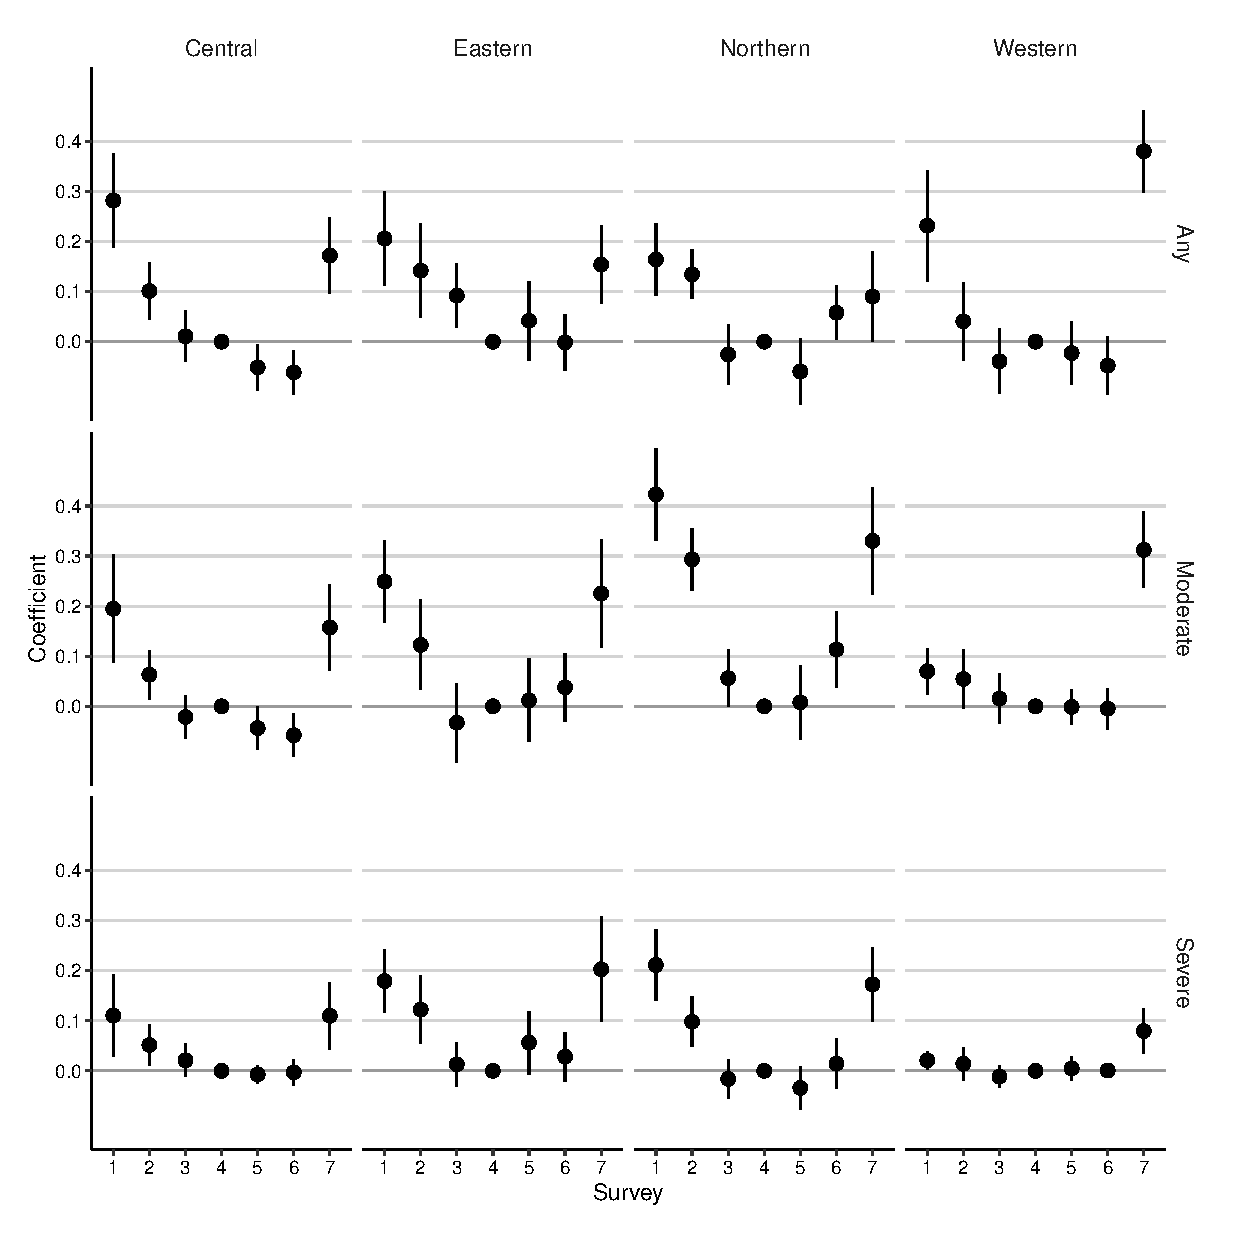
\includegraphics[width=\linewidth, keepaspectratio]{./eps/fig_06.eps}
\end{center}
\figuresource{Authors’ analysis based on data from the Uganda High-Frequency Phone Survey, Rounds 1-7.} 
\figurenote{Household fixed effects estimates relative to Round 4 with each region treated as a separate sample.}
\end{figure}

Both the Central and Eastern regions follow a pattern very closely
aligned with the national-level results. All three levels of food
insecurity are statistically significantly higher in the immediate
aftermath of the first lockdown compared to Round 4, and food insecurity
gradually decrease for the next two survey rounds. The levels remain
approximately constant until after the second lockdown, where food
insecurity levels in Round 7 are all statistically significantly higher
than in Round 4.

For the Northern region, severe food insecurity follows the national
level pattern. However, for moderate/severe food insecurity, only Round
5 is not statistically significantly different from Round 4, and levels
in Rounds 1 and 7 are more than 40 and 30 percentage points higher,
respectively, than Round 4. Furthermore, although the changes in any
food insecurity are closer to the national-level changes, they are
generally smaller.

The Western region is the region that stands out most compared to the
other regions. First, there is little to no change in severe food
insecurity, except for the last survey round, which is just below 10
percentage points higher than Round 4. Similarly, although Rounds 1 and
2 for moderate food insecurity are statistically significantly higher
than Round 4, the effects are smaller than elsewhere. For any food
insecurity, the Round 7 level is substantially larger than any of the
others, despite Round 7 further away from the end of the lockdowns than
Rounds 1 and 2.

What do these regional results tell us about the relative effects of the
lockdowns? There are likely two conflicting dynamics at play here. On
one hand, urbanized areas can more effectively enforce lockdowns, as
shown by the mobility measure for the Central region. On the other hand,
proximity to the poverty line greatly increases vulnerability to food
insecurity. This latter point is crucial, as even minimal enforcement
measures in poorer regions like the Eastern region can precipitate
significant shifts into food insecurity, due to the already precarious
economic standing of these households. This is mirrored in the Northern
region, where, in addition, the high baseline poverty levels mean that
the observed changes in food insecurity are less pronounced over
time---the level of any food insecurity never got below nearly 70\% of
the population at its best.

Finally, the Western region contributed significantly to the high
national-level Round 7 results. Part of this is likely the effect of an
even more prolonged period of below-normal rainfall than the other
regions. Using the Round 2 results as the basis, it appears that about
half of the increase in Round 7 food insecurity is due to the
below-normal rainfall, and the other half is due to the second severe
lockdown, likely combined with the cumulative impact of sustained
lower-level lockdowns in between the most severe lockdowns.

\subsection{The Role of Attrition}\label{the-role-of-attrition}

As discussed above, almost 16\% of the original households surveyed in
Round 1 failed to respond by Round 7. Although new households are added,
a concern is whether the attrition of households is non-random and might
bias the result. To examine how sensitive our results are to attrition,
we perform a bounding exercise, where we either assume that all
households that fail to respond would have been food insecure or that
they would not have been food insecure.\footnote{We would like to thank
  the Editor for this suggestion.}

\begin{figure}
\caption{Food insecurity estimates when assuming that all missing
households are either food insecure or are not food
insecure}\label{fig:attrition}
\begin{center}
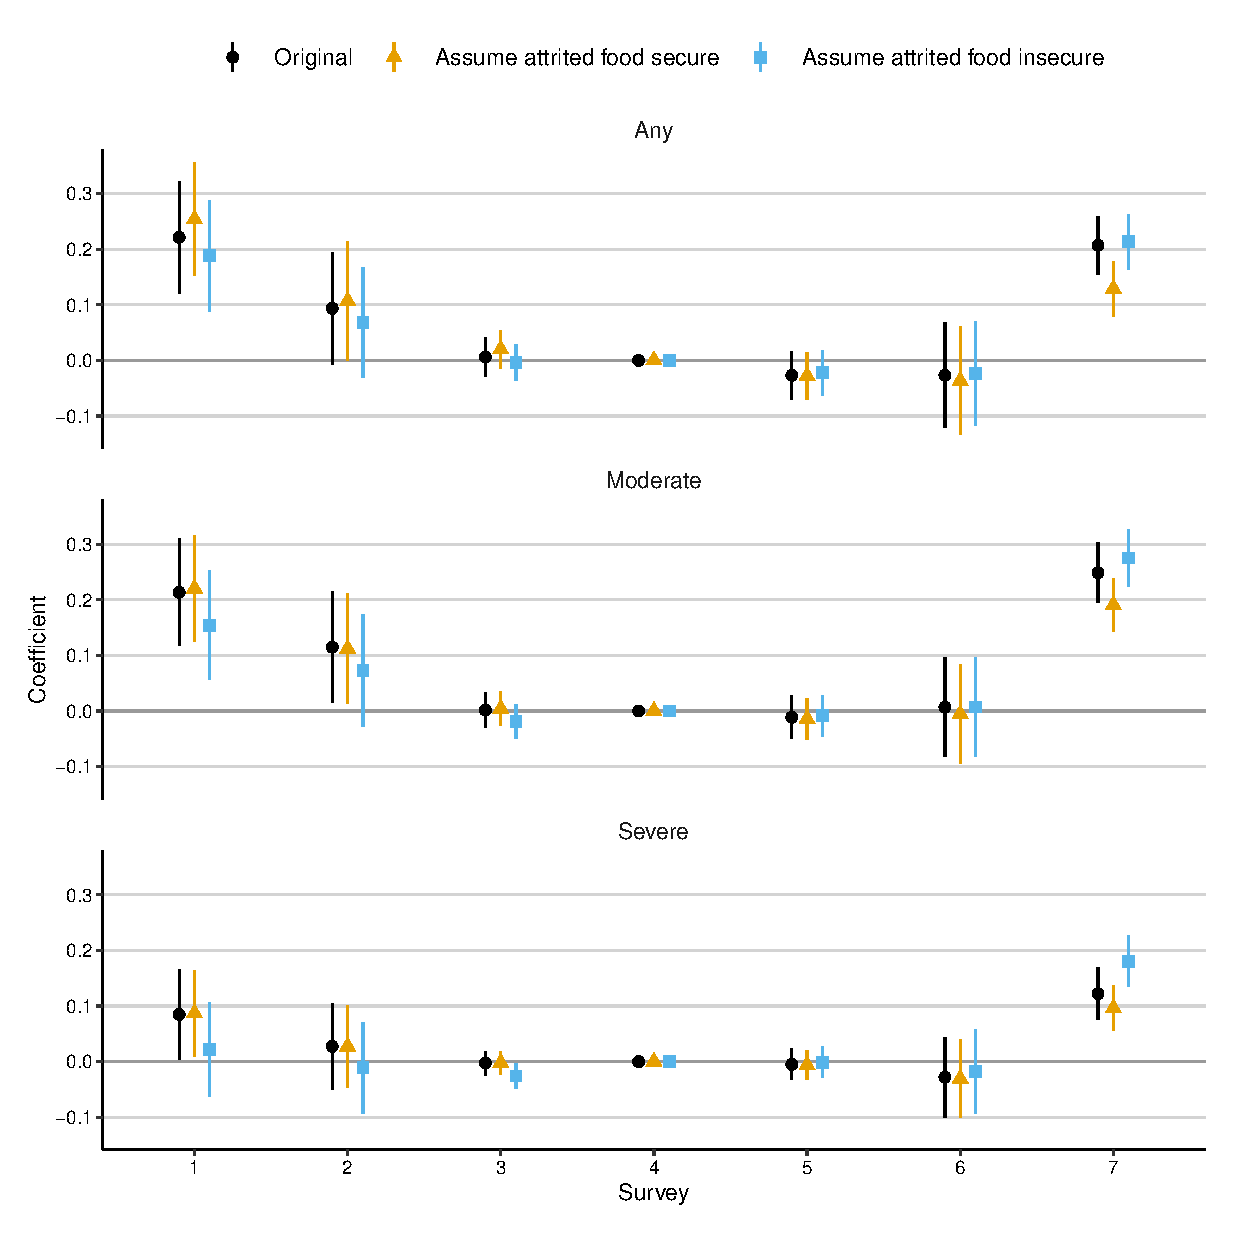
\includegraphics[width=\linewidth, keepaspectratio]{./eps/fig_07.eps}
\end{center}
\figuresource{Authors' analysis based on data from the Uganda High−Frequency Phone Survey, Rounds 1−7.} 
\figurenote{Household fixed effects estimates relative to Round 4. Assume attrited food secure: Estimates when assuming 
    that all missing households would have reported that they were food secure if observed. Assume attrited food insecure:
    Estimates when assuming that all missing households would have reported that they were food insecure if observed.}
\end{figure}

Figure \ref{fig:attrition} shows the results for the nation-wide bounding
estimations together with the original results. For the any and moderate
or severe food insecurity outcomes, whether we assume that attrited
households would have been food insecure or food secure, those results
that were statistically significant in the main model remain
statistically significant for the bounding exercise. The main potential
change in the results is for severe food insecurity in Round 1, where
the first round is no longer statistically significantly different from
Round 4, if we assume that attrition households would have been severely
food insecure, although we cannot reject that the Round 1 coefficients
are the same across the original and the two bounding assumptions.
Furthermore, if we assume severe food insecurity for missing households
the Round 7 estimate is statistically significantly larger than both the
original estimate and the estimate if we assumed that attrited
households were not severely food insecure.

\section{How Households Responded}\label{how-households-responded}

To understand how the government lockdowns affected food insecurity and
how households responded to the lockdowns, we examine four categories:
labor market outcomes, movement between sectors, changes in income
across sources, and assistance from outside sources.

\subsection{Impact on Labor Market Outcomes}\label{impact-on-labor-market-outcomes}

Lockdowns may affect the availability of employment, both because
workplaces close and because of the overall reduction in economic
activity likely to follow lockdowns. Respondents were asked whether they
did ``any work for pay, any kind of business, farming or other activity
to generate income'' in the last week. If yes, they were asked whether
this was the same job as the previous round and the broad industry in
which they worked in the current survey round. For Round 1, respondents
were also asked whether they did the same work as before the pandemic
started and if it was a different job, which industry it was in. We
create two indicator variables to capture the likelihood of working:
doing any market work and working in the same job as the prior round.

The UHFS also asked whether any household member had operated a non-farm
family business since the preceding round, so we also created an
indicator variable where 1 represents operating a business and 0
otherwise. However, Round 1 only asks whether the family has operated a
business since the beginning of 2020 and does not ask about operations
since the start of the lockdown. This means we are unable to use Round 1
information to examine the impact of the lockdown on operating a family
business.

The top three panels of Figure \ref{fig:work_employment} shows the results
for the likelihoods of doing market work, operating a non-farm family
business, and working in the same job as before, using Round 4 as the
base. The bottom two panels show the coefficients for the multinomial
logit model, relative to non-agriculture work, using Round 0,
i.e.\ pre-COVID-19, as the base.

\begin{figure}
\caption{Changes in work and employment outcomes across survey rounds---the top 
three panels show coefficients from linear models with household
fixed effects and dependent indicator variables. The bottom two panels
show coefficients from a fixed effects multinomial logit model, relative
to non-agricultural work.}\label{fig:work_employment}
\begin{center}
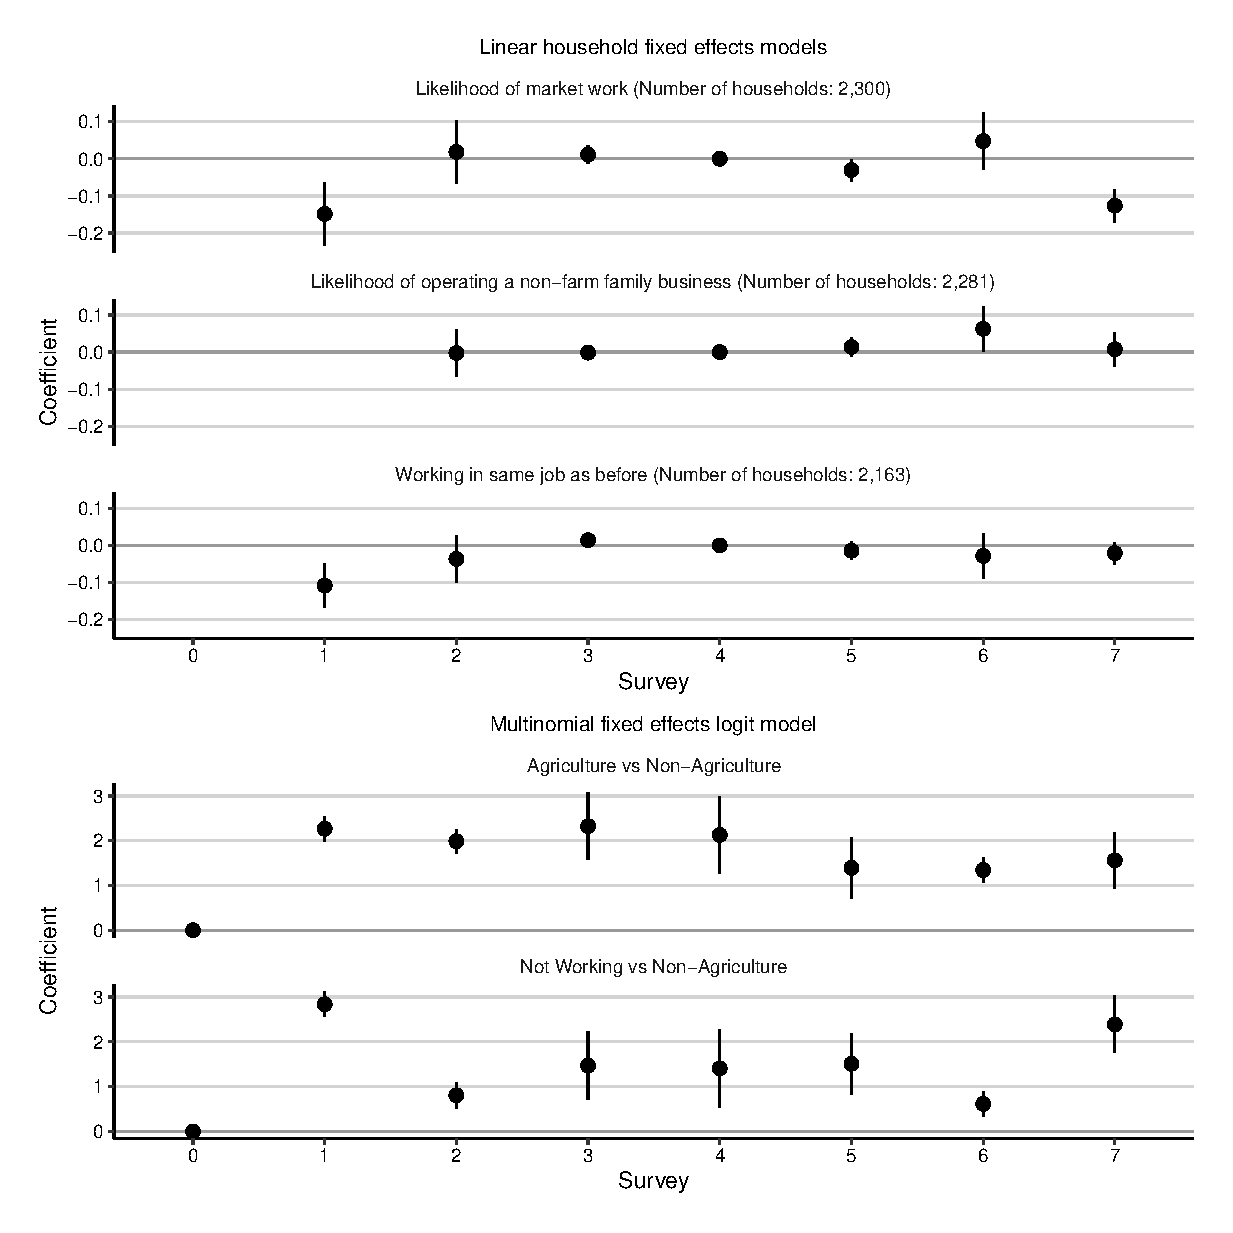
\includegraphics[width=\linewidth, keepaspectratio]{./eps/fig_08.eps}
\end{center}
\figuresource{Authors' analysis based on data from the Uganda High−Frequency Phone Survey, Rounds 1−7.} 
\figurenote{The top 3 panels show coefficients from linear models with household fixed effects. The bottom two panels
    show coefficients from a fixed effects multinomial logit model, relative to non-agricultural work.}
\end{figure}

The likelihood of any market work was significantly lower immediately
after the first lockdown compared to Round 4. Given the very low number
of COVID-19 cases, as shown in Figure \ref{fig:combined}, this effect was
likely driven predominately by the severe lockdown. This is supported by
the stated reasons for not working, which was collected in Round 1; the
top three were that the place of work is closed (62\%), being ill from
any illness or quarantined (10\%), and being laid off from the job
(8\%). Relative to Round 4, there appears to be no medium-run impact of
the first lockdown, although given the absence of information on
pre-Covid we cannot rule out that the levels of market work were
depressed overall.

The medium-run impact of the second lockdown, combined with the
lower-than-normal rainfall is large, with the likelihood of market work
decreasing by around 13 percentage points. This large impact on market
work may explain the large impact on food insecurity in the medium run
following the second lockdown.

We cannot estimate the short-run impact of the lockdown on the
likelihood of operating a non-farm family business, as we do not have
data for Round 1. However, relative to Round 4, the only statistically
significantly coefficient is for Round 6, where there is an
approximately five percentage points higher likelihood of operating a
non-farm business. Combined with the positive, but not statistically
significant coefficient for market work in the same round, this suggests
that the economy had slowly started to recover right before the
beginning of the second severe lockdown.

Given the overall decrease in market work, it is useful to understand
whether individuals who were able to continue working during the
lockdowns did so in the same jobs. The first lockdown was significantly
associated with an approximately 10 percentage points lower likelihood
of working at the same job, relatively to Round 4. Thus, we find both a
decrease in market work and an increased likelihood of moving jobs. The
impact in the medium run is small, indicating that people remained in
their new jobs after the end of the lockdown. There is only a small,
statistically insignificant, effect in the medium run following the
second lockdown. However, we cannot establish whether this is because
the second lockdown follows the same pattern as the first or because
there is less immediate movement compared to the first lockdown.

\subsection{Movement Between Sectors}\label{movement-between-sectors}

With workplace closures during lockdowns and reduced economic activity,
we expect significant movement between the non-agricultural and the
agricultural sectors, and between working and not working. Enforcement
of lockdowns is likely easier in the non-agricultural sector than the
agricultural sector, so we expect that people are more likely to be able
to continue working in the agricultural sector. Furthermore, those who
are laid off may either stop working or resort to agricultural
production at home, even if the income is lower return than in their
original job.

To examine this, we create a three-level categorical variable for the
household's main sector: non-agricultural work (0), agricultural work
(1), and not working (2). We consider a household agricultural if its
main activity was related to agriculture, which includes both farmers,
casual farm laborers, and those employed in any type of processing,
sale, or transport of agricultural goods. These households can be either
urban or rural. As we know the household's main industry prior to the
first lockdown, we have eight rounds of data and use the pre-lockdown
round (i.e., Round 0) as the excluded round.

\begin{table}[hbtp!]
\begin{center}
\begin{footnotesize}
\begin{threeparttable}
\caption{Transition matrices between not working in agriculture, working in agriculture, and not working
by survey round}
\label{tab:transition}
\begin{tabular}{@{} l D{.}{.}{1.2} D{.}{.}{1.2} D{.}{.}{1.2}  D{.}{.}{1.2} D{.}{.}{1.2} D{.}{.}{1.2} @{}}
\toprule 
                & \multicolumn{6}{c}{Current Sector}  \\ \cmidrule(lr){2-7} 
                & \mco{Non-agri-}   & \mco{Agri-}      & \mco{Not}     & \mco{Non-agri-}   & \mco{Agri-}      & \mco{Not}     \\ 
 Prior Sector   & \mco{culture}     & \mco{culture}    & \mco{working} & \mco{culture}     & \mco{culture}    & \mco{working} \\ 
\midrule 
        & \multicolumn{3}{c}{Pre-COVID to Round 1} & \multicolumn{3}{c}{Rounds 1 to 2} \\ \cmidrule(lr){2-4} \cmidrule(lr){5-7} 
Non-agriculture & 0.55 & 0.15 & 0.30 & 0.88 & 0.05 & 0.06 \\ 
 Agriculture & 0.01 & 0.92 & 0.07 & 0.05 & 0.90 & 0.05 \\ 
 Not working & 0.00 & 0.00 & 1.00 & 0.25 & 0.50 & 0.25 \\ 
 \addlinespace
        & \multicolumn{3}{c}{Rounds 2 to 3} & \multicolumn{3}{c}{Rounds 3 to 4} \\ \cmidrule(lr){2-4} \cmidrule(lr){5-7} 
Non-agriculture & 0.93 & 0.01 & 0.06 & 0.94 & 0.03 & 0.03 \\ 
 Agriculture & 0.01 & 0.94 & 0.05 & 0.03 & 0.91 & 0.07 \\ 
 Not working & 0.13 & 0.32 & 0.55 & 0.15 & 0.30 & 0.55 \\ 
 \addlinespace
        & \multicolumn{3}{c}{Rounds 4 to 5} & \multicolumn{3}{c}{Rounds 5 to 6} \\ \cmidrule(lr){2-4} \cmidrule(lr){5-7} 
Non-agriculture & 0.91 & 0.02 & 0.08 & 0.91 & 0.04 & 0.05 \\ 
 Agriculture & 0.04 & 0.82 & 0.14 & 0.03 & 0.90 & 0.07 \\ 
 Not working & 0.14 & 0.21 & 0.65 & 0.10 & 0.41 & 0.49 \\ 
 \addlinespace
        & \multicolumn{3}{c}{Rounds 6 to 7} & \multicolumn{3}{c}{} \\ \cmidrule(lr){2-4}  
Non-agriculture & 0.78 & 0.05 & 0.17 &  &  &  \\ 
 Agriculture & 0.03 & 0.74 & 0.24 &  &  &  \\ 
 Not working & 0.11 & 0.24 & 0.64 &  &  &  \\ 
 \bottomrule
\end{tabular}
\begin{tablenotes}
\item \scriptsize \textit{Source:} Authors' analysis based on data from the Uganda High-Frequency Phone Survey, Rounds 1−7.
\item \scriptsize \textit{Note:} Before COVID-19, there were  868  households in non-agricultural work, 
988  working in agriculture, and  369  not working. 
\end{tablenotes}
\end{threeparttable}
\end{footnotesize}
\end{center}
\end{table}


We use a conditional fixed-effects multinomial logit model to estimate
the movements between agricultural work, non-agricultural work, and not
working. Standard marginal analyses are not meaningful because the
fixed-effects estimator cannot make predictions that account for the
panel-level fixed effects. We, therefore, present the coefficients on
the likelihood of working in the agricultural sector against working in
the non-agricultural sector, and the other is the likelihood of not
working against working in the non-agricultural sector.

The two bottom panels of Figure \ref{fig:work_employment} show the
coefficients for the multinomial fixed effects logit model on the
likelihood of working in the agricultural sector and not working,
respectively, versus working in the non-agricultural sector.
Furthermore, to ease interpretation, Table \ref{tab:transition} shows
the transition probabilities between the three groups from round to
round.\footnote{Figure S4.1 shows the
  unweighted counts of household by labor market group.}

There are two important short-run effects of the first lockdown. First,
there was a significant shift to agriculture from working in the
non-agricultural sector. Second, there is a significant increase in the
risk of not working relative to being employed in the non-agricultural
sector. Only just over half of all households working in the
non-agricultural sector pre-COVID-19 remain in that sector, while 30\%
are not working and 15\% are working in agriculture in Round 1. About
7\% of the households working in agriculture pre-COVID-19 report not
working in Round 1, likely because the lockdowns also affected sale and
processing of agricultural produce. Hence, the results suggest that
while more people were not working, there is also a significant switch
to agricultural work to cope with the effects of the first
lockdown.\footnote{While not focusing on lockdowns, one prior study
  finds evidence that the pandemic itself led to a switch in
  occupations, particularly among salaried and business persons, with
  agriculture seeing the biggest inflow of labor compared to other
  industries \citep{Gupta2021}.}

Although there was some recovery by Round 2, half of those who were not
working in Round 1 are now working in agriculture, while only 25\% move
(back) to the non-agricultural sector. Furthermore, relative to
pre-COVID-19, households remain substantially more likely to be working
in agriculture than non-agriculture for the next three survey rounds,
and only by Round 5, March 2021, is there a reduction in the likelihood
of working in agriculture, although it comes not from a movement to
non-agricultural work but rather from not working.

Unfortunately, we cannot see the short-term movement across groups after
the second lockdown, but the medium-term effect is a reversal of the
very gradual improvement in the likelihood of working in the
non-agricultural sector that occurred between Round 2 and 6. This is
combined with a substantial movement to not working, mostly from
agriculture, possibly from a combination of the lockdown and the
lower-than-normal rainfall. The lack of opportunities in the
agricultural sector may also explain why individuals were likely to
remain at the same job after the second lockdown (Panel 3).

The results suggest that the COVID-19 lockdowns had pronounced effects
on employment dynamics, underscored by the migration from
non-agricultural to agricultural employment and the significant
increases in the likelihood of not working. Furthermore, after the first
lockdown, those who could continue working were significantly more
likely to work in new jobs, some of which were likely in agriculture. We
do not have direct information on wages. However, these new jobs likely
paid less than the pre-lockdown job, given the economy's contraction,
the increasing supply of workers relative to available openings, and the
movement toward the agricultural sector, where the marginal product of
an additional worker is likely to be low. The high rate of new jobs and
the reduction in movements between jobs after the first lockdown suggest
continued labor market difficulties in the medium run, which would also
affect food insecurity.

Although there was a semblance of recovery after the first lockdown, the
continued high levels of agricultural employment imply a structural
rather than a transitory adjustment to the employment landscape.
Furthermore, the resurgence of restrictions interrupted the nascent
recovery in non-agricultural employment, showing the precariousness of
economic revival in the face of additional lockdowns. Overall, the
results underscore the agricultural sector's role as a vital reservoir
of employment during periods of economic upheaval, yet also highlight
its susceptibility to further disruptions, whether policy-driven or
environmental.

\subsection{Income Sources}\label{income-sources}

Households were asked questions related to income in Rounds 1 through 6.
Rather than the monetary value of their income, households were asked
whether their income from different sources increased, remained the
same, decreased, or was completely lost since the prior round (for Round
1, the questions were asked relative to the start date of the lockdown).
The income questions covered five sources: (i) family farming,
livestock, or fishing, (ii) non-farm family business, (iii) wage
employment, (iv) income from assets (properties, investments, or
savings), and (v) pension. As the income question was ordinal, we
created variables for each income source where 1 represents an increase
in income, 0 represents income remaining unchanged, and -1 represents a
decrease in income or a complete loss.

\begin{figure}
\caption{Impact on the levels of income from farms, non-farm businesses,
wages, and assets---coefficients from fixed effects ordered logit
model, with positive representing an increase, 0 no change, and negative
a decrease}\label{fig:income_sources}
\begin{center}
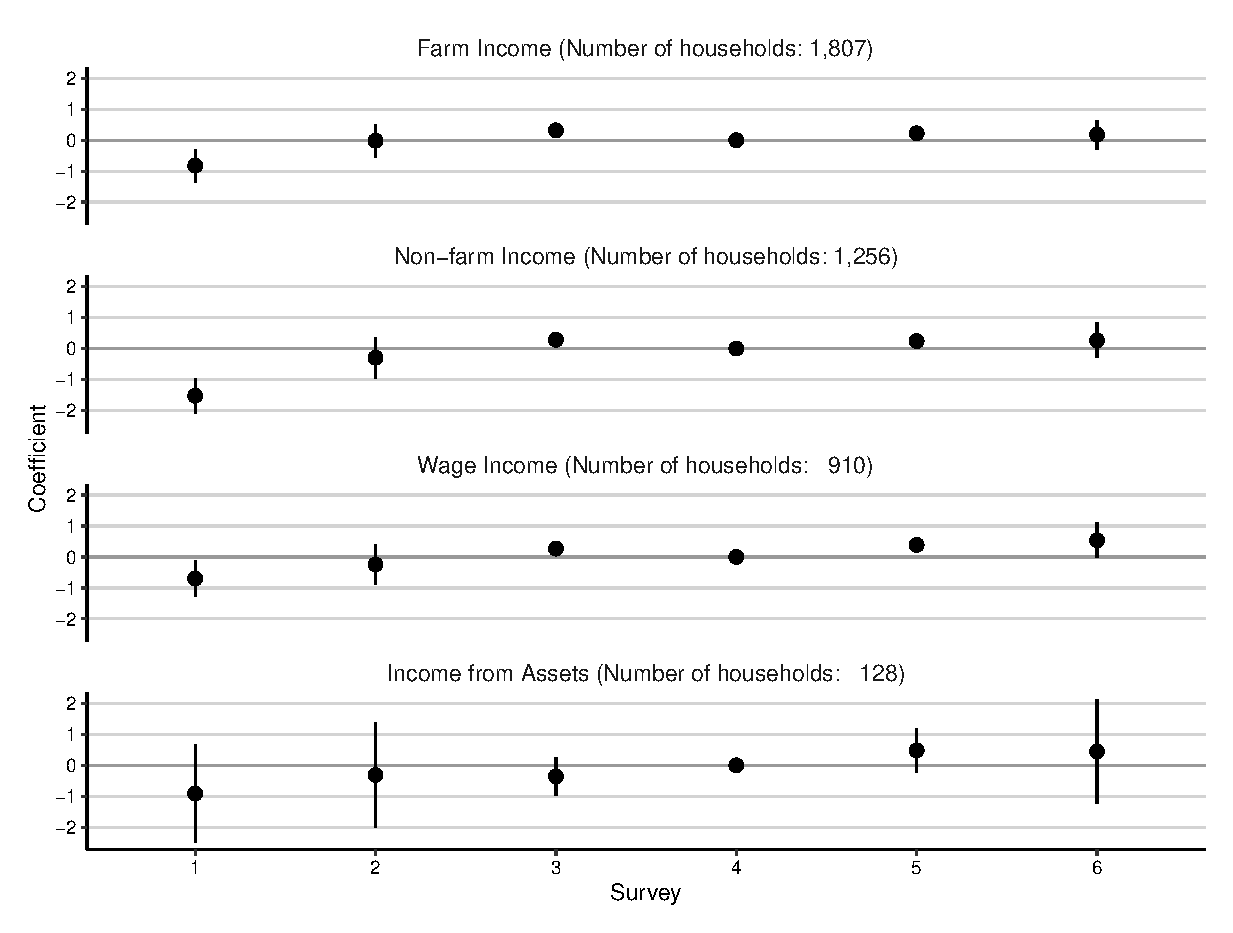
\includegraphics[width=\linewidth, keepaspectratio]{./eps/fig_09.eps}
\end{center}
\figuresource{Authors' analysis based on data from the Uganda High−Frequency Phone Survey, Rounds 1−7.} 
\figurenote{Coefficients from fixed effects ordered logit model, with positive representing 
an increase, 0 no change, and negative a decrease.}
\end{figure}

Given that we use ordinal variables to represent changes in household
income, we use a conditional fixed-effects ordered logistic model. The
typical conditional logit model works by applying a fixed-effects logit
model for households that see a change in the dependent variable over
time. For the conditional \emph{ordered} logit model, the actual values
of the dependent variable are irrelevant. Instead, greater values
correspond to higher-value outcomes \citep{Baetschmann2015}. Hence, for
our regressions, a positive coefficient for lockdowns represents an
increase in household income, a negative coefficient represents a
decrease, and a coefficient near 0 indicates that income remained
stable. The results are shown in Figure \ref{fig:income_sources} together
with the number of households that the estimations are based
on.\footnote{Only 34 households ever reported pension income, so we do
  not show results for this income source.}

The first lockdown significantly decreased farm income, non-farm income,
and wage income. Furthermore, the effect on income from assets is
negative, although not statistically significant, likely because of the
low number of households who own assets.

The effects persisted in the medium run, with very few households
reporting improvements between Rounds 1 and 2, and, as a consequence,
the estimated effects are either zero or negative. Only by the third
round do a significant number of households report improvements in
income levels. We do not have income data for Round 7 and thus cannot
examine the medium-term impact of the second lockdown. These income
effects are likely a major reason for the significant increase in food
insecurity from the lockdowns.

\subsection{Outside Assistance}\label{outside-assistance}

Given the reductions in household income with the lockdowns, we examine
potential coping mechanisms in this section and the next
\citep{Morduch1995, Townsend1994}.

Households may, for example, rely on assistance from family members
outside the household or from institutions. In rounds 1 through 6, the
UHFS asked households whether they received assistance from the
following sources: (i) remittance from abroad, (ii) assistance from
family members within the country, (iii) assistance from other
non-family individuals, (iv) assistance from NGOs, and (v) assistance
from the government.\footnote{Households were also asked whether they
  received unemployment benefits, but there was only one observation
  with a change in level, so we do not have any variation to conduct a
  conditional ordered logit estimation.} The questions were asked the
same way as the income questions, where households can either report
income increase, remaining the same, decrease, or complete loss relative
to the prior round. Therefore, like the income estimations, we create
ordinal variables where 1, 0, and -1 represent an increase, same, and
decrease/complete loss, respectively, and estimate the effect of
lockdowns using the same conditional fixed-effects ordered logistic
model. The results are shown in Figure \ref{fig:income_assistance}.

\begin{figure}
\caption{Impact on the level of outside assistance---coefficients from
fixed effects ordered logit model, with positive representing an
increase, 0 no change, and negative a
decrease}\label{fig:income_assistance}
\begin{center}
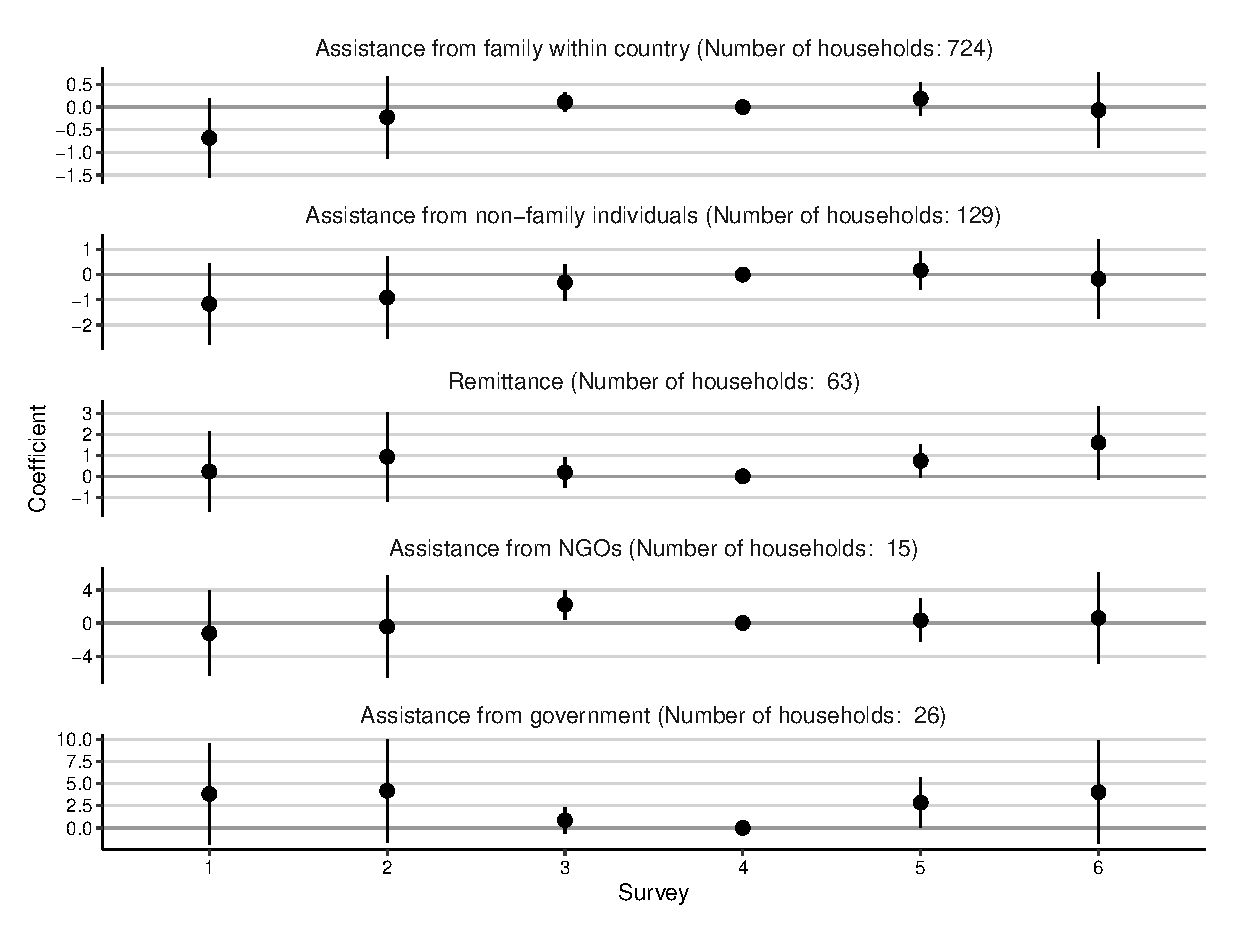
\includegraphics[width=\linewidth, keepaspectratio]{./eps/fig_10.eps}
\end{center}
\figuresource{Authors' analysis based on data from the Uganda High−Frequency Phone Survey, Rounds 1−7.} 
\figurenote{Coefficients from fixed effects ordered logit model, with positive representing an increase, 0 no change, and
    negative a decrease.}
\end{figure}

We find no statistically significant effect on the assistance from
family with the country, assistance from non-family individuals, or
remittances after the first lockdown. The first two fell slightly, while
the level of remittances increased slightly. This statistically
insignificant increase for remittances does run counter to the
substantial decline in remittances across the world in the second
quarter of 2020, as lockdowns worldwide led to the closure of workplaces
and limited people's movements
\citep{Cardozo-Silva2022, Guha2021, Kpodar2023, Shimizutani2021, Zhang2021}.
However, only 63 households reported any change over the six survey
rounds.

Neither could the households turn to NGOs or the government for help.
Only 15 households report any change in NGO assistance, while only 26
households report a change in government assistance. Not surprisingly,
both coefficients are very noisy for the first and second rounds.

These results suggest that households' standard coping mechanisms were
unavailable during the lockdowns. The failure of these coping mechanisms
in the face of reductions in income likely contributed substantially to
the large effects of lockdowns on food insecurity.

\subsection{Other Changes to the Household}\label{other-changes-to-the-household}

As households faced greater food insecurity during lockdowns, it is
possible that, on the one hand, some household members left to look for
better opportunities. On the other hand, lockdowns resulted in decreased
income and diminished work opportunities, and schools were closed
throughout the entire period. Consequently, migrants may have chosen to
return to their families, and students attending boarding
schools---particularly common in secondary education---also likely
returned home, and these returns may further increase food
insecurity.\footnote{Children at local schools would also spend more
  time at home more as a result of the school closures. Although we
  cannot directly capture this dimension, it is likely that it added to
  the general level of food insecurity as these children often would
  have been served lunch at school, as was the case for Nigeria
  \citep{Abay2021}.}

Using the household rosters from UHFS and the UNPS 2019/20, we have data
on the number of household members, adults, and children, and location
of the households for the last UNPS survey before COVID-19, here
referred to as Round 0, and for each survey round. One caveat is that
UNPS 2019/20 data collection took place between April 2019 and February
2020, which means that the pre-COVID-19 information on household size
can be more than a year for the first UHFS survey. The top three panels
of Figure \ref{fig:members_location} show the impact of lockdowns on the
number of household members and on the number of adults and children
separately.

\begin{figure}
\caption{Impact on the number of household members and the likelihood of
urban locations --- household fixed effects coefficients from linear
models with continuous outcome variables for the top three panels and an
indicator variable for the bottom panel.}\label{fig:members_location}
\begin{center}
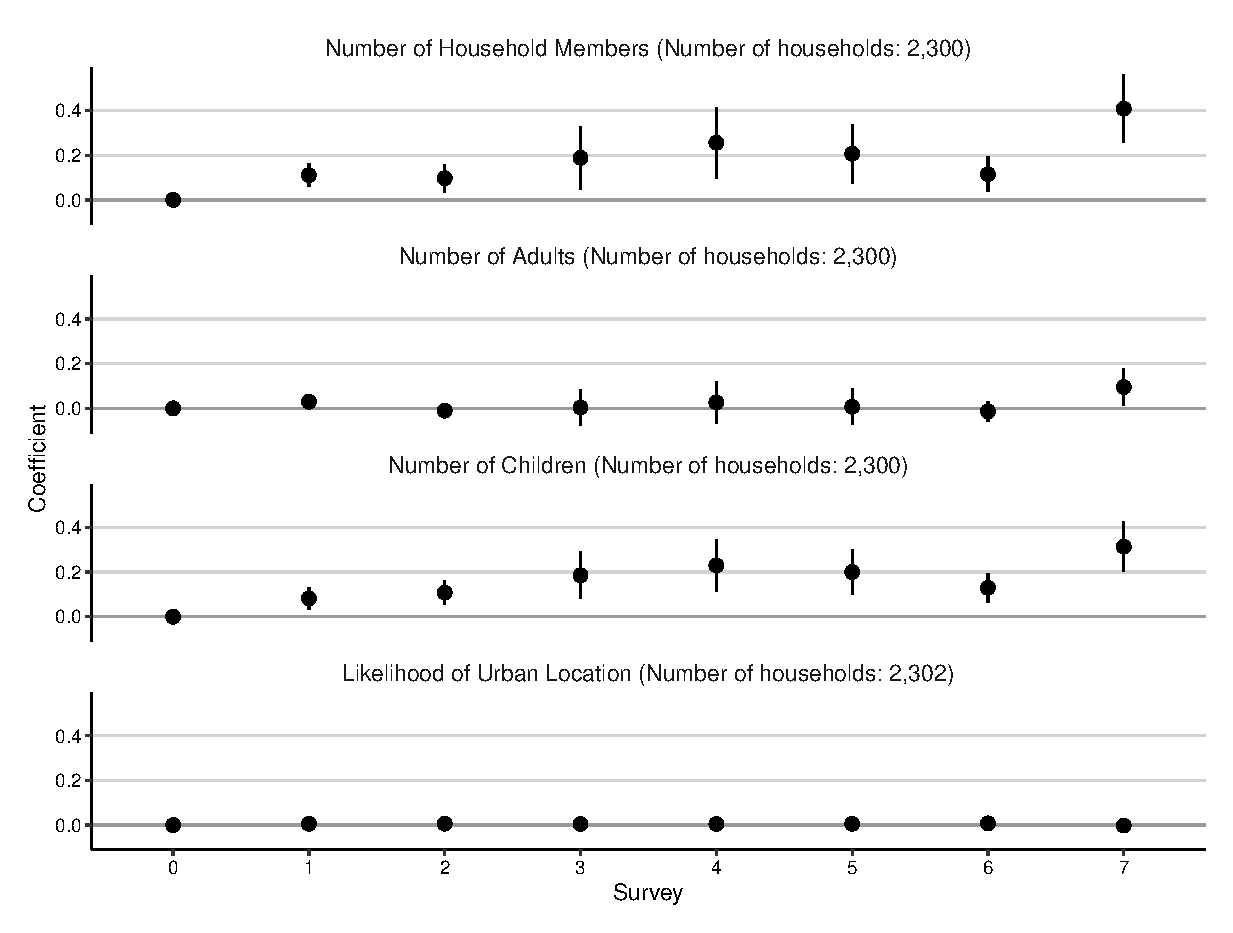
\includegraphics[width=\linewidth, keepaspectratio]{./eps/fig_11.eps}
\end{center}
\figuresource{Authors' analysis based on data from the Uganda High−Frequency Phone Survey, Rounds 1−7.} 
\figurenote{Coefficients from household fixed effects coefficients from linear models with continuous outcome variables for 
    the top three panels and an indicator variable for the bottom panel.}
\end{figure}

Relatively to before COVID-19, the number of household members is
statistically significantly higher throughout the entire period. This
effect comes almost entirely from an increase in the number of children.
The exception is for Round 7, where there are statistically significant
increases in both the number of adults and the number of children,
relatively to before COVID-19. The continuous increase in the number of
children until Round 4 compared to the pre-COVID-19 survey, suggests
that this change is not driven by the lockdowns and school closures,
which began at the same time as the first lockdown and did not end until
2022.

Hence, although the school closures may have increased the base level of
food insecurity compared to before COVID-19, it is unlikely to have
driven the increases in food insecurity during the first lockdowns.

The relative reduction in household size in Round 6 may be related to
the improvement of the labor market suggested above with older children
moving to jobs. However, similarly to the likelihood of market work, the
second lockdown reversed the positive trend, substantially increasing
the number of both adult and young household members.

Related to migration, we find no such evidence of lockdown-induced
migration in the bottom panel of Figure \ref{fig:members_location}, which
shows the likelihood of living in an urban area.

Lastly, given the shift to agricultural work, we examine whether
agricultural households change their agricultural strategy to cope with
the lockdowns. We find suggestive evidence that agricultural households
changed their farming strategy during the lockdowns, such as changing
the farming area and changes in the variety of crops produced. 
The details of these results are in the Online Appendix.

Overall, our results indicate that the households, on average, could not
take advantage of outside help, whether it was assistance from family
members living outside of the household or assistance from institutions.
We do find evidence of a switch to agricultural work.

\subsection{Agricultural vs. Non-Agricultural Households}\label{agricultural-vs.-non-agricultural-households}

Given the increase in agricultural work with the first lockdown,
Figure \ref{fig:ag_vs_non_ag} examines whether agricultural households
fared better than non-agricultural households. We show the results for
two different approaches. First, the two left columns separate
households by whether they were agricultural households before COVID-19
and estimate each level of food insecurity.\footnote{Round 1 of the
  survey asks about the household's area of work before the lockdown,
  which allows us to identify whether households were in agriculture
  before the first lockdown.} Second, the results in the right two
columns come from one regression per level of food insecurity and use
the prior rounds' reported agricultural status interacted with the
survey indicators. Note, as we previously treated households' work in
agriculture as a choice variable, this set of estimations is exploratory
rather than causal. In all cases, the effects are shown relative to
survey Round 4 as above.

\begin{figure}
\caption{Estimated changes in food insecurity with 95\% confidence
intervals by survey round relative to Round 4, controlling for household
fixed effects, for non-agricultural and agricultural households. Left
two columns condition on pre-COVID-19 agricultural status, while the
right two columns allow households to change
status}\label{fig:ag_vs_non_ag}
\begin{center}
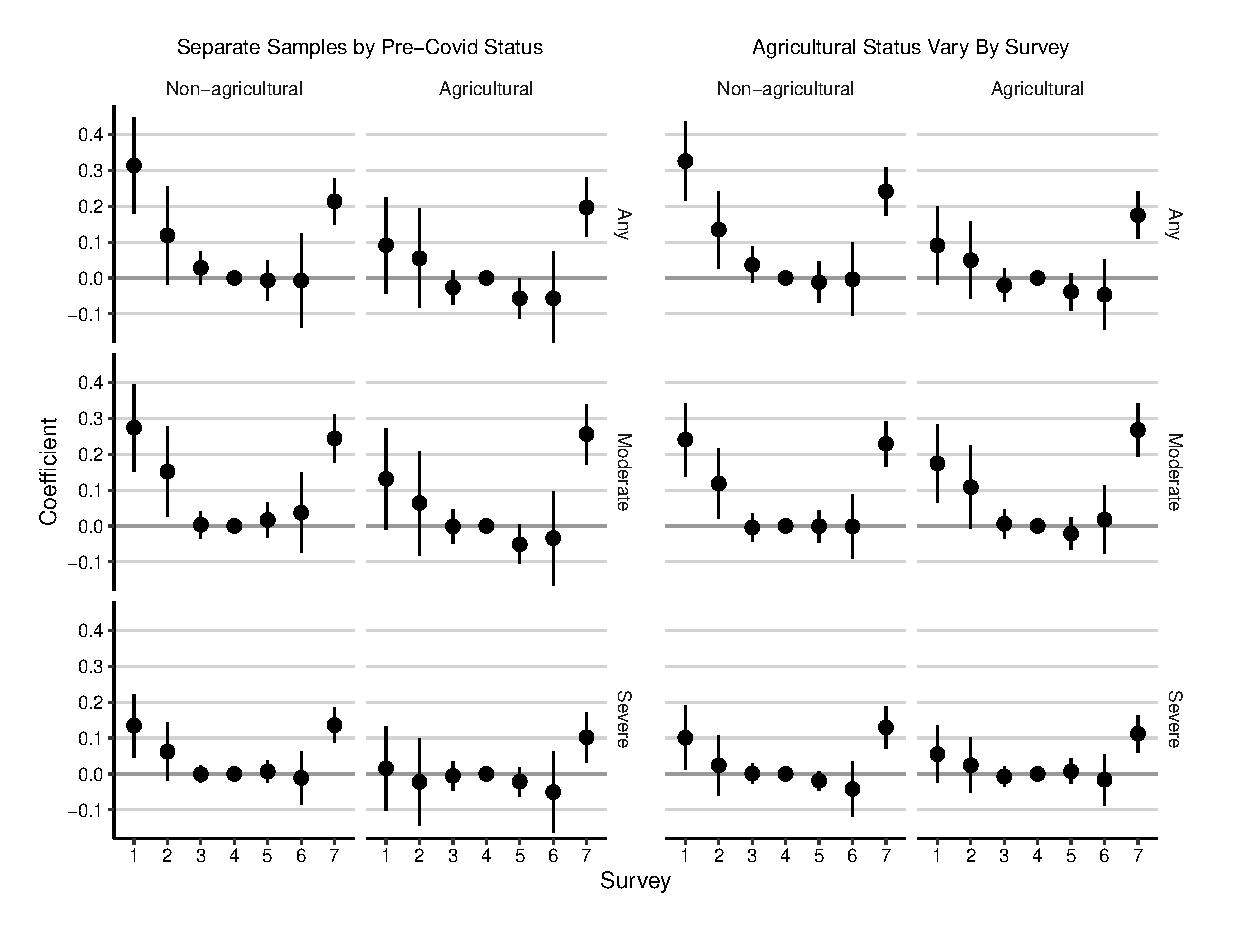
\includegraphics[width=\linewidth, keepaspectratio]{./eps/fig_12.eps}
\end{center}
\figuresource{Authors' analysis based on data from the Uganda High−Frequency Phone Survey, Rounds 1−7.} 
\figurenote{Coefficients from household fixed effects models for non-agricultural and agricultural households. Left two columns 
    condition on pre-COVID-19 agricultural status, while the right two columns allow households to change status.}
\end{figure}


Agricultural households' food security changed less than
non-agricultural households' food security during the first lockdown.
Their likelihood of suffering ``any food insecurity'' during lockdowns,
relative to Round 4, was about 20 percentage points lower than
non-agricultural households, as shown by Round 1. In fact, there are no
statistically significant differences between Rounds 1 and 4 for
agricultural households, whether we use pre-COVID-19 or prior survey
agricultural status. Agricultural households also do better than
non-agricultural households when it comes to both moderate/severe or
severe food insecurity, although the difference is less stark for these
outcomes. Specifically, for severe food insecurity, the estimated
difference between Round 1 and 4 is very close to zero.

However, for Round 7, there is little difference across different
measures of food insecurity, with all groups seeing statistically
significant increases in food insecurity. This suggests that the
concurrent lower-than-normal rainfall removed some of the protection
from lockdowns that agricultural households had previously had.

\section{Conclusion}\label{conclusion}

As countries around the world continue to navigate the challenges posed
by the aftermath of the COVID-19 pandemic and plan for responses to
potential future crises and epidemics, understanding the cost and
benefits of potential policies is critical. Using country-wide panel
data with a household fixed-effects model, we examine the impact of the
two COVID-19 lockdowns in Uganda on food insecurity and household
responses. As we use the periods during COVID-19 with fewer restrictions
as the comparison, we expect our results to be lower-bound estimates.

Food insecurity increased substantially during the first lockdown. The
first lockdown also had a significant medium-run impact on food
insecurity. The medium-run impact was even more pronounced following the
second lockdown. The larger effect is likely partly from the compounding
effect of the concurrent environmental stressors of a lower-than-normal
rainfall, especially in the Western region of Uganda, and partly from
reduced resilience after the effects of the first lockdown.

The lockdowns led to significant disruptions in income sources across
the board, with decreases in income from agriculture, non-farm
businesses, and wage employment contributing to the rise in food
insecurity. Both agricultural and non-agricultural households were
affected, although non-agricultural households experienced more severe
impacts. This difference underscores the relative resilience of
agricultural activities during lockdown periods. Agriculture provided a
coping mechanism for many households, and the switch towards
agricultural work suggests a strategic shift in employment patterns in
response to the lockdown measures.

However, traditional sources of coping mechanisms, such as reliance on
outside assistance from family members and friends, NGOs, or government
support, proved inadequate during the lockdowns, leaving households to
face the economic shocks with limited external support. Remittance from
abroad, assistance from family members within the country, assistance
from non-family individuals, and assistance from development
organizations, were all either flat or decreased during the lockdowns.
This lack of assistance may explain lockdowns' substantial effect on
food insecurity.

Three broader conclusions emerge from our results. First, on average,
agriculture is likely less productive than non-farm work but more
productive than not working. Hence, with the slow rate of switching back
from agriculture that we observe, the lockdowns can potentially have
severe long-term adverse effects on Uganda's development.

Second, the results show the limits of self-insurance and mutual
insurance when faced with a systemic shock. Most of the literature has
focused on the smaller and more frequent risk of idiosyncratic shocks
and how households respond to these. However, a better understanding of
systemic shocks and how households respond is still lacking.

Finally, the case of Uganda illustrates well the issues with the
wholesale lockdown of economies in response to COVID-19, particularly in
situations with low state capacity. Uganda has been hailed as a leading
example of curbing COVID-19 \citep{Adams2021}. However, the mitigation
efforts failed to reach those most affected by the lockdown. With the
low mortality rate in Sub-Saharan Africa, including Uganda, the
long-term cost of the lockdowns likely significantly outweighs the
benefits. In addition to the increasing food insecurity and decline in
economic activity, the lockdowns disrupted education and reduced
accessibility and use of health care with the lockdowns in
Uganda.\footnote{See \citet{Bose2023} on health care and
  \citet{Batte2021} for an early assessment of the effects on education
  on a small sample.} Quantifying all these costs and identifying
possible avenues of mitigation are critical future areas of research.




\appendix
\setcounter{section}{1}

\appsection{Household Surveyed in UHFS}



\begin{table}[hbtp!]
\begin{center}
\begin{small}
\begin{threeparttable}
\caption{Number of Original and New Households by Survey Round}
\label{tab:surveys}
\begin{tabular}{@{} l rrrrrrr @{}}
\toprule 
       & \multicolumn{7}{c}{Survey Round} \\ \cmidrule(lr){2-8} 
        & 1 & 2 & 3 & 4 & 5 & 6 & 7 \\ 
\midrule 
Original Households & 2,225 & 2,145 & 2,091 & 2,083 & 2,067 & 2,038 & 1,873 \\ 
 New Households in Round &   0 &  44 &  41 &   3 &   6 &   5 &  10 \\ 
 Total Households Surveyed & 2,225 & 2,189 & 2,169 & 2,127 & 2,112 & 2,089 & 1,927 \\ 
 \bottomrule
\end{tabular}
\begin{tablenotes}
\scriptsize
\item {\it Source:} Authors' analysis based on data from the Uganda High-Frequency Phone Survey, Rounds 1−7.
\item {\it Note:} Original households are households 
surveyed in the first round. New households are households added as replacements.
\end{tablenotes}
\end{threeparttable}
\end{small}
\end{center}
\end{table}

\bibliographystyle{wber}

\begin{thebibliography}{}

\bibitem[\protect\citeauthoryear{Abay, Amare, Tiberti, and Andam}{Abay
  et~al.}{2021}]{Abay2021}
Abay, K.~A., M.~Amare, L.~Tiberti, and K.~S. Andam. 2021.
\newblock ``Covid-19-induced disruptions of school feeding services exacerbate
  food insecurity in {Nigeria}.''
\newblock {\em The Journal of Nutrition\/}~{ 151\/}~(8): 2245--2254.

\bibitem[\protect\citeauthoryear{Adams, MacKenzie, Amegah, Ezeh, Gadanya,
  Omigbodun, Sarki, Thistle, Ziraba, Stranges, and Silverman}{Adams
  et~al.}{2021}]{Adams2021}
Adams, J., M.~J. MacKenzie, A.~K. Amegah, A.~Ezeh, M.~A. Gadanya, A.~Omigbodun,
  A.~M. Sarki, P.~Thistle, A.~K. Ziraba, S.~Stranges, and M.~Silverman. 2021.
\newblock ``The {Conundrum} of {Low} {COVID}-19 {Mortality} {Burden} in
  sub-{Saharan} {Africa}: {Myth} or {Reality}?.''
\newblock {\em Global Health: Science and Practice\/}~{ 9\/}~(3): 433--443.
\newblock Publisher: Global Health: Science and Practice \_eprint:
  https://www.ghspjournal.org/content/9/3/433.full.pdf.

\bibitem[\protect\citeauthoryear{Agamile}{Agamile}{2022}]{Agamile2022}
Agamile, P. 2022, December.
\newblock ``{COVID}-19 {Lockdown} and {Exposure} of {Households} to {Food}
  {Insecurity} in {Uganda}: {Insights} from a {National} {High} {Frequency}
  {Phone} {Survey}.''
\newblock {\em The European Journal of Development Research\/}~{34}:
  3050--3075.

\bibitem[\protect\citeauthoryear{Aggarwal, Jeong, Kumar, Park, Robinson, and
  Spearot}{Aggarwal et~al.}{2022}]{Aggarwal2022}
Aggarwal, S., D.~Jeong, N.~Kumar, D.~S. Park, J.~Robinson, and A.~Spearot.
  2022.
\newblock ``{COVID}-19 market disruptions and food security: {Evidence} from
  households in rural {Liberia} and {Malawi}.''
\newblock {\em PloS One\/}~{ 17\/}~(8): e0271488.

\bibitem[\protect\citeauthoryear{Alam and Bose}{Alam and Bose}{2020}]{Alam2020}
Alam, S.~A., and B.~Bose. 2020.
\newblock ``Did the {Great} {Recession} {Affect} {Fertility}? {Examining} the
  {Impact} of {Job} {Displacements} on the {Timing} of {Births} in the {United}
  {States}.''
\newblock {\em Southern Economic Journal\/}~{ 86\/}~(3): 873--909.
\newblock \_eprint: https://onlinelibrary.wiley.com/doi/pdf/10.1002/soej.12408.

\bibitem[\protect\citeauthoryear{Alam, Liu, and P{\"o}rtner}{Alam
  et~al.}{2024}]{Alam2024}
Alam, S.~A., S.~X. Liu, and C.~C. P{\"o}rtner. 2024, Oct.
\newblock ``Navigating food price shocks in a pandemic: Food insecurity and
  coping mechanisms in {Burkina Faso}.''
\newblock {\em World Development\/}~{182}: 106714.

\bibitem[\protect\citeauthoryear{Alam and P{\"o}rtner}{Alam and
  P{\"o}rtner}{2018}]{Alam2018}
Alam, S.~A., and C.~C. P{\"o}rtner. 2018, March.
\newblock ``Income shocks, contraceptive use, and timing of fertility.''
\newblock {\em Journal of Development Economics\/}~{131}: 96--103.
\newblock Publisher: Elsevier B.V.

\bibitem[\protect\citeauthoryear{Alfonsi, Bandiera, Bassi, Burgess, Rasul,
  Veroux, and Vitali}{Alfonsi et~al.}{2021}]{Alfonsi2021}
Alfonsi, L., O.~Bandiera, V.~Bassi, R.~Burgess, I.~Rasul, O.~Veroux, and
  A.~Vitali. 2021, October.
\newblock ``{COVID}-19 and {Ugandan} {SMEs}: {Impacts} and {Speed} of
  {Recovery}.''.
\newblock Policy Brief UGA-20273, International Growth Centre.

\bibitem[\protect\citeauthoryear{Amare, Abay, Tiberti, and Chamberlin}{Amare
  et~al.}{2021}]{Amare2021}
Amare, M., K.~A. Abay, L.~Tiberti, and J.~Chamberlin. 2021, May.
\newblock ``{COVID}-19 and food security: {Panel} data evidence from
  {Nigeria}.''
\newblock {\em Food Policy\/}~{101}: 102099.

\bibitem[\protect\citeauthoryear{Atamanov, Cochinard, Ilukor, Kilic, and
  Ponzini}{Atamanov et~al.}{2022}]{Atamanov2022}
Atamanov, A., F.~Cochinard, J.~Ilukor, T.~Kilic, and G.~Ponzini. 2022, March.
\newblock ``Economic impact of a second lockdown in {Uganda}: results from the
  seventh round of the {High}-{Frequency} {Phone} {Survey}.''.

\bibitem[\protect\citeauthoryear{Athumani}{Athumani}{2021}]{Athumani2021}
Athumani, H. 2021.
\newblock ``Uganda {Lifts} {Some} {COVID}-19 {Restrictions}.''.

\bibitem[\protect\citeauthoryear{Baetschmann, Staub, and
  Winkelmann}{Baetschmann et~al.}{2015}]{Baetschmann2015}
Baetschmann, G., K.~E. Staub, and R.~Winkelmann. 2015.
\newblock ``Consistent estimation of the fixed effects ordered logit model.''
\newblock {\em Journal of the Royal Statistical Society. Series A (Statistics
  in Society)\/}~{ 178\/}~(3): 685--703.
\newblock Publisher: [Wiley, Royal Statistical Society].

\bibitem[\protect\citeauthoryear{Balde, Boly, and Avenyo}{Balde
  et~al.}{2021}]{Balde2021}
Balde, R., M.~Boly, and E.~Avenyo. 2021, Jan.
\newblock ``Labour market effects of covid-19 in sub-saharan africa: An
  informality lens from burkina faso, mali and senegal.''
\newblock {\em Revue d'{\'e}conomie du d{\'e}veloppement\/}~{ 29\/}~(1-2):
  43--84.

\bibitem[\protect\citeauthoryear{Batte, Semulimi, Mutebi, Mukisa, Olum, and
  Bongomin}{Batte et~al.}{2021}]{Batte2021}
Batte, C., A.~W. Semulimi, R.~K. Mutebi, J.~Mukisa, R.~Olum, and F.~Bongomin.
  2021, Jul.
\newblock ``Assessment of the impact of covid-19 pandemic on the education and
  psychosocial wellbeing of school-going children in {Bududa} {District},
  {Uganda}.''.
\newblock Technical report.

\bibitem[\protect\citeauthoryear{BBC}{BBC}{2020}]{BBC2020}
BBC. 2020, July.
\newblock ``Uganda - where security forces may be more deadly than
  coronavirus.''.

\bibitem[\protect\citeauthoryear{Birner, Blaschke, Bosch, Daum, Graf,
  G{\"u}ttler, Heni, Kariuki, Katusiime, Seidel, Senon, and Woode}{Birner
  et~al.}{2021}]{Birner2021}
Birner, R., N.~Blaschke, C.~Bosch, T.~Daum, S.~Graf, D.~G{\"u}ttler, J.~Heni,
  J.~Kariuki, R.~Katusiime, A.~Seidel, Z.~N. Senon, and G.~Woode. 2021,
  December.
\newblock ```{We} would rather die from {Covid}-19 than from hunger' -
  {Exploring} lockdown stringencies in five {African} countries.''
\newblock {\em Global Food Security\/}~{31}: 100571.

\bibitem[\protect\citeauthoryear{Biryabarema}{Biryabarema}{2021}]{Biryabarema2021}
Biryabarema, E. 2021, July.
\newblock ``Uganda partially eases {COVID}-19 containment measures.''.

\bibitem[\protect\citeauthoryear{Bose, Alam, and P{\"o}rtner}{Bose
  et~al.}{2023}]{Bose2023}
Bose, B., S.~A. Alam, and C.~C. P{\"o}rtner. 2023, September.
\newblock ``{Impacts of the COVID-19 Lockdown on Healthcare Inaccessibility and
  Unaffordability in Uganda}.''
\newblock {\em American Journal of Tropical Medicine and Hygiene\/}~{
  109\/}~(3): 527--535.

\bibitem[\protect\citeauthoryear{Cardozo~Silva, Diaz~Pavez,
  Mart{\'\i}nez‐Zarzoso, and Nowak‐Lehmann}{Cardozo~Silva
  et~al.}{2022}]{Cardozo-Silva2022}
Cardozo~Silva, A.~R., L.~R. Diaz~Pavez, I.~Mart{\'\i}nez‐Zarzoso, and
  F.~Nowak‐Lehmann. 2022, May.
\newblock ``The impact of {COVID}‐19 government responses on remittances in
  {Latin} {American} countries.''
\newblock {\em Journal of International Development\/}~{ 34\/}~(4): 803--822.
\newblock Publisher: John Wiley and Sons Ltd.

\bibitem[\protect\citeauthoryear{Ceballos, Hernandez, and Paz}{Ceballos
  et~al.}{2021}]{Ceballos2021a}
Ceballos, F., M.~A. Hernandez, and C.~Paz. 2021, May.
\newblock ``Short‐term impacts of {COVID}‐19 on food security and nutrition
  in rural {Guatemala}: {Phone}‐based farm household survey evidence.''
\newblock {\em Agricultural Economics\/}~{ 52\/}~(3): 477--494.
\newblock Number: 3.

\bibitem[\protect\citeauthoryear{Ceballos, Kannan, and Kramer}{Ceballos
  et~al.}{2020}]{Ceballos2020}
Ceballos, F., S.~Kannan, and B.~Kramer. 2020, December.
\newblock ``Impacts of a national lockdown on smallholder farmers' income and
  food security: {Empirical} evidence from two states in {India}.''
\newblock {\em World Development\/}~{136}: 105069.

\bibitem[\protect\citeauthoryear{Ceballos, Kannan, and Kramer}{Ceballos
  et~al.}{2021}]{Ceballos2021}
Ceballos, F., S.~Kannan, and B.~Kramer. 2021.
\newblock ``Crop prices, farm incomes, and food security during the {COVID}-19
  pandemic in {India}: {Phone}-based producer survey evidence from {Haryana}
  {State}.''
\newblock {\em Agricultural Economics\/}~{ 52\/}~(3): 525--542.
\newblock Number: 3 \_eprint:
  https://onlinelibrary.wiley.com/doi/pdf/10.1111/agec.12633.

\bibitem[\protect\citeauthoryear{Charles and DeCicca}{Charles and
  DeCicca}{2008}]{Charles2008}
Charles, K.~K., and P.~DeCicca. 2008, December.
\newblock ``Local labor market fluctuations and health: {Is} there a connection
  and for whom?.''
\newblock {\em Journal of Health Economics\/}~{ 27\/}~(6): 1532--1550.

\bibitem[\protect\citeauthoryear{Curi-Quinto, S{\'a}nchez, Lago-Berrocal,
  Penny, Murray, Nunes, Favara, Wijeyesekera, Lovegrove, Soto-C{\'a}ceres, and
  Vimaleswaran}{Curi-Quinto et~al.}{2021}]{Curi-Quinto2021}
Curi-Quinto, K., A.~S{\'a}nchez, N.~Lago-Berrocal, M.~E. Penny, C.~Murray,
  R.~Nunes, M.~Favara, A.~Wijeyesekera, J.~A. Lovegrove, V.~Soto-C{\'a}ceres,
  and K.~S. Vimaleswaran. 2021, October.
\newblock ``Role of {Government} {Financial} {Support} and {Vulnerability}
  {Characteristics} {Associated} with {Food} {Insecurity} during the {COVID}-19
  {Pandemic} among {Young} {Peruvians}.''
\newblock {\em Nutrients\/}~{ 13\/}~(10): 3546.

\bibitem[\protect\citeauthoryear{Dasgupta and Robinson}{Dasgupta and
  Robinson}{2021}]{Dasgupta2021}
Dasgupta, S., and E.~J.~Z. Robinson. 2021, September.
\newblock ``Food {Insecurity}, {Safety} {Nets}, and {Coping} {Strategies}
  during the {COVID}-19 {Pandemic}: {Multi}-{Country} {Evidence} from
  {Sub}-{Saharan} {Africa}.''
\newblock {\em International Journal of Environmental Research and Public
  Health\/}~{ 18\/}~(19): 9997.

\bibitem[\protect\citeauthoryear{Del~Ninno, Dorosh, and Smith}{Del~Ninno
  et~al.}{2003}]{Del-Ninno2003}
Del~Ninno, C., P.~A. Dorosh, and L.~C. Smith. 2003, July.
\newblock ``Public {Policy}, {Markets} and {Household} {Coping} {Strategies} in
  {Bangladesh}: {Avoiding} a {Food} {Security} {Crisis} {Following} the 1998
  {Floods}.''
\newblock {\em Economic Crises, Natural Disasters, and Poverty\/}~{ 31\/}~(7):
  1221--1238.

\bibitem[\protect\citeauthoryear{Deshpande}{Deshpande}{2020}]{Deshpande2020}
Deshpande, A. 2020, Jul.
\newblock ``The {Covid}-19 {Pandemic} and {Lockdown}: {First} {Order} {Effects}
  on {Gender} {Gaps} in {Employment} and {Domestic} {Time} {Use} in {India}.''.
\newblock GLO Discussion Paper Series 607, Global Labor Organization (GLO),
  Essen, Germany.

\bibitem[\protect\citeauthoryear{Djomaleu, Rogers, Barrie, Rutherford, Weiser,
  and Kelly}{Djomaleu et~al.}{2022}]{Djomaleu2022}
Djomaleu, M.~L., A.~B. Rogers, M.~B. Barrie, G.~W. Rutherford, S.~D. Weiser,
  and J.~D. Kelly. 2022, 10.
\newblock ``Long-term consequences of food insecurity among ebola virus
  disease-affected households after the 2013--2016 epidemic in rural
  communities of kono district, sierra leone: A qualitative study.''
\newblock {\em PLOS Global Public Health\/}~{ 2\/}~(10): 1--16.

\bibitem[\protect\citeauthoryear{Egger, Miguel, Warren, Shenoy, Collins,
  Karlan, Parkerson, Mobarak, Fink, Udry, Walker, Haushofer, Larreboure, Athey,
  Lopez-Pena, Benhachmi, Humphreys, Lowe, Meriggi, Wabwire, Davis, Pape, Graff,
  Voors, Nekesa, and Vernot}{Egger et~al.}{2022}]{Egger2022}
Egger, D., E.~Miguel, S.~S. Warren, A.~Shenoy, E.~Collins, D.~Karlan,
  D.~Parkerson, A.~M. Mobarak, G.~Fink, C.~Udry, M.~Walker, J.~Haushofer,
  M.~Larreboure, S.~Athey, P.~Lopez-Pena, S.~Benhachmi, M.~Humphreys, L.~Lowe,
  N.~F. Meriggi, A.~Wabwire, C.~A. Davis, U.~J. Pape, T.~Graff, M.~Voors,
  C.~Nekesa, and C.~Vernot. 2022, April.
\newblock ``Falling living standards during the {COVID}-19 crisis:
  {Quantitative} evidence from nine developing countries.''
\newblock {\em Science Advances\/}~{ 7\/}~(6): eabe0997.
\newblock Number: 6 Publisher: American Association for the Advancement of
  Science.

\bibitem[\protect\citeauthoryear{Fallon and Lucas}{Fallon and
  Lucas}{2002}]{Fallon2002}
Fallon, P.~R., and R.~E.~B. Lucas. 2002, May.
\newblock ``The {Impact} of {Financial} {Crises} on {Labor} {Markets},
  {Household} {Incomes}, and {Poverty}: {A} {Review} of {Evidence}.''
\newblock {\em The World Bank Research Observer\/}~{ 17\/}~(1): 21--45.

\bibitem[\protect\citeauthoryear{FAO}{FAO}{2015}]{FAO2015}
FAO. 2015.
\newblock ``Modeling food insecurity in bivariate and regression analyses.''.
\newblock Technical report, {Food and Agricultural Organization of the United
  Nations}, Rome, Italy.

\bibitem[\protect\citeauthoryear{FAO}{FAO}{2016}]{FAO2016}
FAO. 2016.
\newblock ``Methods for estimating comparable prevalence rates of food
  insecurity experienced by adults throughout the world.''.
\newblock Technical report, {Food and Agricultural Organization of the United
  Nations}, Rome, Italy.

\bibitem[\protect\citeauthoryear{FAO}{FAO}{2022}]{FAO2022}
FAO. 2022, October.
\newblock ``{GIEWS} {Country} {Brief} - {Uganda}.''.
\newblock Technical report, Food and Agricultural Organization of the United
  Nations.

\bibitem[\protect\citeauthoryear{Foster and Rosenzweig}{Foster and
  Rosenzweig}{2002}]{Foster2002}
Foster, A.~D., and M.~R. Rosenzweig. 2002, October.
\newblock ``Household {Division} and {Rural} {Economic} {Growth}.''
\newblock {\em The Review of Economic Studies\/}~{ 69\/}~(4): 839--869.

\bibitem[\protect\citeauthoryear{Gait{\'a}n-Rossi, Vilar-Compte, Teruel, and
  P{\'e}rez-Escamilla}{Gait{\'a}n-Rossi et~al.}{2021}]{Gaitan-Rossi2021}
Gait{\'a}n-Rossi, P., M.~Vilar-Compte, G.~Teruel, and R.~P{\'e}rez-Escamilla.
  2021, February.
\newblock ``Food insecurity measurement and prevalence estimates during the
  {COVID}-19 pandemic in a repeated cross-sectional survey in {Mexico}.''
\newblock {\em Public Health Nutrition\/}~{ 24\/}~(3): 412--421.
\newblock Number: 3.

\bibitem[\protect\citeauthoryear{Gatiso, Ordaz-N{\'e}meth, Grimes, Lormie,
  Tweh, K{\"u}hl, and Junker}{Gatiso et~al.}{2018}]{Gatiso2018}
Gatiso, T.~T., I.~Ordaz-N{\'e}meth, T.~Grimes, M.~Lormie, C.~Tweh, H.~S.
  K{\"u}hl, and J.~Junker. 2018, 08.
\newblock ``The impact of the ebola virus disease (evd) epidemic on
  agricultural production and livelihoods in liberia.''
\newblock {\em PLOS Neglected Tropical Diseases\/}~{ 12\/}~(8): 1--17.

\bibitem[\protect\citeauthoryear{Giacoman, Herrera, and
  Ayala~Arancibia}{Giacoman et~al.}{2021}]{Giacoman2021}
Giacoman, C., M.~Herrera, and P.~Ayala~Arancibia. 2021, September.
\newblock ``Household food insecurity before and during the {COVID}-19 pandemic
  in {Chile}.''
\newblock {\em Public Health\/}~{198}: 332--339.

\bibitem[\protect\citeauthoryear{Glewwe and Hall}{Glewwe and
  Hall}{1998}]{Glewwe1998}
Glewwe, P., and G.~Hall. 1998, June.
\newblock ``Are some groups more vulnerable to macroeconomic shocks than
  others? {Hypothesis} tests based on panel data from {Peru}.''
\newblock {\em Journal of Development Economics\/}~{ 56\/}~(1): 181--206.

\bibitem[\protect\citeauthoryear{Google}{Google}{2022}]{Google2022}
Google. 2022.
\newblock ``{COVID}-19 {Community} {Mobility} {Report}.''.

\bibitem[\protect\citeauthoryear{Guha, Islam, and Hussain}{Guha
  et~al.}{2021}]{Guha2021}
Guha, P., B.~Islam, and M.~A. Hussain. 2021.
\newblock ``{COVID}-19 lockdown and penalty of joblessness on income and
  remittances: {A} study of inter-state migrant labourers from {Assam},
  {India}.''
\newblock {\em Journal of Public Affairs\/}~{ 21\/}~(4): e2470.
\newblock \_eprint: https://onlinelibrary.wiley.com/doi/pdf/10.1002/pa.2470.

\bibitem[\protect\citeauthoryear{Guloba, Kakuru, and Ssewanyana}{Guloba
  et~al.}{2021}]{Guloba2021}
Guloba, M.~M., M.~Kakuru, and S.~N. Ssewanyana. 2021, July.
\newblock ``The impact of {COVID}-19 on industries without smokestacks in
  {Uganda}.''.
\newblock Technical report, Africa Growth Initiative at Brookings.

\bibitem[\protect\citeauthoryear{Gupta, Malani, and Woda}{Gupta
  et~al.}{2021}]{Gupta2021}
Gupta, A., A.~Malani, and B.~Woda. 2021, June.
\newblock ``Explaining the {Income} and {Consumption} {Effects} of {COVID} in
  {India}.''.
\newblock NBER Working Paper 28935, National Bureau of Economic Research.
\newblock Issue: 28935 Series: Working Paper Series.

\bibitem[\protect\citeauthoryear{Hallegatte, Vogt-Schilb, Rozenberg, Bangalore,
  and Beaudet}{Hallegatte et~al.}{2020}]{Hallegatte2020}
Hallegatte, S., A.~Vogt-Schilb, J.~Rozenberg, M.~Bangalore, and C.~Beaudet.
  2020, April.
\newblock ``From {Poverty} to {Disaster} and {Back}: a {Review} of the
  {Literature}.''
\newblock {\em Economics of Disasters and Climate Change\/}~{ 4\/}~(1):
  223--247.

\bibitem[\protect\citeauthoryear{Hamadani, Hasan, Baldi, Hossain, Shiraji,
  Bhuiyan, Mehrin, Fisher, Tofail, Tipu, Grantham-McGregor, Biggs, Braat, and
  Pasricha}{Hamadani et~al.}{2020}]{Hamadani2020}
Hamadani, J.~D., M.~I. Hasan, A.~J. Baldi, S.~J. Hossain, S.~Shiraji, M.~S.~A.
  Bhuiyan, S.~F. Mehrin, J.~Fisher, F.~Tofail, S.~M. M.~U. Tipu,
  S.~Grantham-McGregor, B.-A. Biggs, S.~Braat, and S.-R. Pasricha. 2020,
  November.
\newblock ``Immediate impact of stay-at-home orders to control {COVID}-19
  transmission on socioeconomic conditions, food insecurity, mental health, and
  intimate partner violence in {Bangladeshi} women and their families: an
  interrupted time series.''
\newblock {\em The Lancet. Global Health\/}~{ 8\/}~(11): e1380--e1389.

\bibitem[\protect\citeauthoryear{Harris, Depenbusch, Pal, Nair, and
  Ramasamy}{Harris et~al.}{2020}]{Harris2020}
Harris, J., L.~Depenbusch, A.~A. Pal, R.~M. Nair, and S.~Ramasamy. 2020.
\newblock ``Food system disruption: initial livelihood and dietary effects of
  {COVID}-19 on vegetable producers in {India}.''
\newblock {\em Food Security\/}~{ 12\/}~(4): 841--851.

\bibitem[\protect\citeauthoryear{Himelein, Testaverde, Turay, and
  Turay}{Himelein et~al.}{2015}]{Himelein2015}
Himelein, K., M.~Testaverde, A.~Turay, and S.~Turay. 2015, Jun.
\newblock ``The socio-economic impacts of ebola in {Sierra Leone}: results from
  a high frequency cell phone survey (round three).''.
\newblock Working paper, World Bank, Washington, D.C.

\bibitem[\protect\citeauthoryear{Hirvonen, de~Brauw, and Abate}{Hirvonen
  et~al.}{2021}]{Hirvonen2021}
Hirvonen, K., A.~de~Brauw, and G.~T. Abate. 2021.
\newblock ``Food {Consumption} and {Food} {Security} during the {COVID}-19
  {Pandemic} in {Addis} {Ababa}.''
\newblock {\em American Journal of Agricultural Economics\/}~{ 103\/}~(3):
  772--789.

\bibitem[\protect\citeauthoryear{Jaacks, Veluguri, Serupally, Roy, Prabhakaran,
  and Ramanjaneyulu}{Jaacks et~al.}{2021}]{Jaacks2021}
Jaacks, L.~M., D.~Veluguri, R.~Serupally, A.~Roy, P.~Prabhakaran, and
  G.~Ramanjaneyulu. 2021, October.
\newblock ``Impact of the {COVID}-19 pandemic on agricultural production,
  livelihoods, and food security in {India}: baseline results of a phone
  survey.''
\newblock {\em Food Security\/}~{ 13\/}~(5): 1323--1339.

\bibitem[\protect\citeauthoryear{Janssens, Pradhan, de~Groot, Sidze, Donfouet,
  and Abajobir}{Janssens et~al.}{2021}]{Janssens2021}
Janssens, W., M.~Pradhan, R.~de~Groot, E.~Sidze, H.~P.~P. Donfouet, and
  A.~Abajobir. 2021, February.
\newblock ``The short-term economic effects of {COVID}-19 on low-income
  households in rural {Kenya}: {An} analysis using weekly financial household
  data.''
\newblock {\em World Development\/}~{138}: 105280.

\bibitem[\protect\citeauthoryear{Jayachandran}{Jayachandran}{2006}]{Jayachandran2006}
Jayachandran, S. 2006.
\newblock ``Selling {Labor} {Low}: {Wage} {Responses} to {Productivity}
  {Shocks} in {Developing} {Countries}.''
\newblock {\em Journal of Political Economy\/}~{ 114\/}~(3): 538--575.

\bibitem[\protect\citeauthoryear{Kang, Baidya, Aaron, Wang, Chan, and
  Wetzler}{Kang et~al.}{2021}]{Kang2021}
Kang, Y., A.~Baidya, A.~Aaron, J.~Wang, C.~Chan, and E.~Wetzler. 2021,
  December.
\newblock ``Differences in the early impact of {COVID}-19 on food security and
  livelihoods in rural and urban areas in the {Asia} {Pacific} {Region}.''
\newblock {\em Global Food Security\/}~{31}: 100580.

\bibitem[\protect\citeauthoryear{Kansiime, Tambo, Mugambi, Bundi, Kara, and
  Owuor}{Kansiime et~al.}{2021}]{Kansiime2021}
Kansiime, M.~K., J.~A. Tambo, I.~Mugambi, M.~Bundi, A.~Kara, and C.~Owuor.
  2021, January.
\newblock ``{COVID}-19 implications on household income and food security in
  {Kenya} and {Uganda}: {Findings} from a rapid assessment.''
\newblock {\em World Development\/}~{137}: 105199.

\bibitem[\protect\citeauthoryear{Kesar, Abraham, Lahoti, Nath, and
  Basole}{Kesar et~al.}{2021}]{Kesar2021}
Kesar, S., R.~Abraham, R.~Lahoti, P.~Nath, and A.~Basole. 2021, April.
\newblock ``Pandemic, informality, and vulnerability: impact of {COVID}-19 on
  livelihoods in {India}.''
\newblock {\em Canadian Journal of Development Studies / Revue canadienne
  d'{\'e}tudes du d{\'e}veloppement\/}~{ 42\/}~(1-2): 145--164.

\bibitem[\protect\citeauthoryear{Kochar}{Kochar}{1999}]{Kochar1999}
Kochar, A. 1999, Feb.
\newblock ``{Smoothing Consumption by Smoothing Income: Hours-of-Work Responses
  to Idiosyncratic Agricultural Shocks in Rural India}.''
\newblock {\em Review of Economics and Statistics\/}~{ 81\/}~(1): 50--61.

\bibitem[\protect\citeauthoryear{Komin, Thepparp, Subsing, and Engstrom}{Komin
  et~al.}{2021}]{Komin2021}
Komin, W., R.~Thepparp, B.~Subsing, and D.~Engstrom. 2021, April.
\newblock ``Covid-19 and its impact on informal sector workers: a case study of
  {Thailand}.''
\newblock {\em Asia Pacific Journal of Social Work and Development\/}~{
  31\/}~(1-2): 80--88.

\bibitem[\protect\citeauthoryear{Kpodar, Mlachila, Quayyum, and
  Gammadigbe}{Kpodar et~al.}{2023}]{Kpodar2023}
Kpodar, K., M.~Mlachila, S.~Quayyum, and V.~Gammadigbe. 2023.
\newblock ``Defying the odds: Remittances during the covid-19 pandemic.''
\newblock {\em The Journal of Development Studies\/}~{ 59\/}~(5): 673--690.

\bibitem[\protect\citeauthoryear{Kundu, Banna, Sayeed, Sultana, Brazendale,
  Harris, Mandal, Jahan, Abid, and Khan}{Kundu et~al.}{2021}]{Kundu2021}
Kundu, S., M.~H.~A. Banna, A.~Sayeed, M.~S. Sultana, K.~Brazendale, J.~Harris,
  M.~Mandal, I.~Jahan, M.~T. Abid, and M.~S.~I. Khan. 2021, April.
\newblock ``Determinants of household food security and dietary diversity
  during the {COVID}-19 pandemic in {Bangladesh}.''
\newblock {\em Public Health Nutrition\/}~{ 24\/}~(5): 1079--1087.

\bibitem[\protect\citeauthoryear{Langlay}{Langlay}{2014}]{Langlay2014}
Langlay, N. 2014, Dec.
\newblock ``The impact of {Ebola} virus disease on village savings and loans
  associations {Montserrado}, {Margibi}, {Bong} and {Lofa} counties.''.
\newblock Technical report, {Food and Agricultural Organization of the United
  Nations}.

\bibitem[\protect\citeauthoryear{Lee, Sahai, Baylis, and Greenstone}{Lee
  et~al.}{2022}]{Lee2022}
Lee, K., H.~Sahai, P.~Baylis, and M.~Greenstone. 2022, May.
\newblock ``Job loss and behavioral change: The unprecedented effects of the
  {India} lockdown in {Delhi}.''.
\newblock BFI Working Paper 2020-65, Becker Friedman Institute for Economics at
  the University of Chicago, Chicago, IL.

\bibitem[\protect\citeauthoryear{Mahmud and Riley}{Mahmud and
  Riley}{2021}]{Mahmud2021}
Mahmud, M., and E.~Riley. 2021, April.
\newblock ``Household response to an extreme shock: {Evidence} on the immediate
  impact of the {Covid}-19 lockdown on economic outcomes and well-being in
  rural {Uganda}.''
\newblock {\em World Development\/}~{140}: 105318.

\bibitem[\protect\citeauthoryear{Mahmud and Riley}{Mahmud and
  Riley}{2023}]{Mahmud2023}
Mahmud, M., and E.~Riley. 2023, March.
\newblock ``Adapting to an aggregate shock: {The} impact of the {Covid}-19
  crisis on rural households.''
\newblock {\em Review of Economics of the Household\/}~{ 21\/}~(1): 19--36.

\bibitem[\protect\citeauthoryear{{Makerere University School of Statistics and
  Planning}}{{Makerere University School of Statistics and
  Planning}}{2023}]{Makerere-University-School-of-Statistics-and-Planning2023}
{Makerere University School of Statistics and Planning}. 2023, Feb.
\newblock ``Socio-economic impact of the {Ebola} virus disease outbreak on
  household welfare: The case of {Kassanda} and {Mubende} districts in
  {Uganda}.''.
\newblock Technical report, United Nations Children's Fund Uganda, Kampala,
  Uganda.

\bibitem[\protect\citeauthoryear{Margini, Pattnaik, Jordanwood, Nakyanzi, and
  Byakika}{Margini et~al.}{2020}]{Margini2020}
Margini, F., A.~Pattnaik, T.~Jordanwood, A.~Nakyanzi, and S.~Byakika. 2020.
\newblock ``Case study: {The} {Initial} {COVID}-19 response in {Uganda}.''.
\newblock Technical report, ThinkWell and Ministry of Health Uganda,
  Washington, DC.

\bibitem[\protect\citeauthoryear{McKenzie}{McKenzie}{2003}]{McKenzie2003}
McKenzie, D.~J. 2003, July.
\newblock ``How do {Households} {Cope} with {Aggregate} {Shocks}? {Evidence}
  from the {Mexican} {Peso} {Crisis}.''
\newblock {\em Economic Crises, Natural Disasters, and Poverty\/}~{ 31\/}~(7):
  1179--1199.

\bibitem[\protect\citeauthoryear{Monitor}{Monitor}{2020}]{Monitor2020}
Monitor. 2020, July.
\newblock ``Gulu {District} lockdown to be lifted on {Monday}.''.

\bibitem[\protect\citeauthoryear{Morduch}{Morduch}{1995}]{Morduch1995}
Morduch, J. 1995.
\newblock ``Income {Smoothing} and {Consumption} {Smoothing}.''
\newblock {\em Journal of Economic Perspectives\/}~{ 9\/}~(3): 103--114.

\bibitem[\protect\citeauthoryear{Nguyen, Kachwaha, Pant, Tran, Ghosh, Sharma,
  Shastri, Escobar-Alegria, Avula, and Menon}{Nguyen
  et~al.}{2021}]{Nguyen2021a}
Nguyen, P.~H., S.~Kachwaha, A.~Pant, L.~M. Tran, S.~Ghosh, P.~K. Sharma, V.~D.
  Shastri, J.~Escobar-Alegria, R.~Avula, and P.~Menon. 2021, April.
\newblock ``Impact of {COVID}-19 on household food insecurity and interlinkages
  with child feeding practices and coping strategies in {Uttar} {Pradesh},
  {India}: a longitudinal community-based study.''
\newblock {\em BMJ open\/}~{ 11\/}~(4): e048738.

\bibitem[\protect\citeauthoryear{Pitt, Rosenzweig, and Hassan}{Pitt
  et~al.}{1990}]{Pitt1990}
Pitt, M.~M., M.~R. Rosenzweig, and M.~N. Hassan. 1990.
\newblock ``{Productivity, Health, and Inequality in the Intrahousehold
  Distribution of Food in Low-Income Countries}.''
\newblock {\em American Economic Review\/}~{ 80\/}~(5): 1139--1156.

\bibitem[\protect\citeauthoryear{R{\"o}nkk{\"o}, Rutherford, and
  Sen}{R{\"o}nkk{\"o} et~al.}{2022}]{Ronkko2022}
R{\"o}nkk{\"o}, R., S.~Rutherford, and K.~Sen. 2022, January.
\newblock ``The impact of the {COVID}-19 pandemic on the poor: {Insights} from
  the {Hrishipara} diaries.''
\newblock {\em World Development\/}~{149}: 105689.

\bibitem[\protect\citeauthoryear{Ruszczyk, Rahman, Bracken, and Sudha}{Ruszczyk
  et~al.}{2021}]{Ruszczyk2021}
Ruszczyk, H.~A., M.~F. Rahman, L.~J. Bracken, and S.~Sudha. 2021, April.
\newblock ``Contextualizing the {COVID}-19 pandemic's impact on food security
  in two small cities in {Bangladesh}.''
\newblock {\em Environment and Urbanization\/}~{ 33\/}~(1): 239--254.

\bibitem[\protect\citeauthoryear{Schotte, Danquah, Osei, and Sen}{Schotte
  et~al.}{2023}]{Schotte2023}
Schotte, S., M.~Danquah, R.~D. Osei, and K.~Sen. 2023, Apr.
\newblock ``The labour market impact of {COVID-19} lockdowns: Evidence from
  {Ghana}.''
\newblock {\em Journal of African Economies\/}~{ 32\/}~(Supplement 2):
  ii10--ii33.

\bibitem[\protect\citeauthoryear{Schwartz, Muddu, Kimera, Mbuliro, Ssennyonjo,
  Ssinabulya, and Semitala}{Schwartz et~al.}{2021}]{Schwartz2021}
Schwartz, J.~I., M.~Muddu, I.~Kimera, M.~Mbuliro, R.~Ssennyonjo, I.~Ssinabulya,
  and F.~C. Semitala. 2021, February.
\newblock ``Impact of a {COVID}-19 {National} {Lockdown} on {Integrated} {Care}
  for {Hypertension} and {HIV}.''
\newblock {\em Global Heart\/}~{ 16\/}~(1): 9.

\bibitem[\protect\citeauthoryear{Shimizutani and Yamada}{Shimizutani and
  Yamada}{2021}]{Shimizutani2021}
Shimizutani, S., and E.~Yamada. 2021, September.
\newblock ``Resilience against the pandemic: {The} impact of {COVID}-19 on
  migration and household welfare in {Tajikistan}.''
\newblock {\em PLOS ONE\/}~{ 16\/}~(9).
\newblock Publisher: Public Library of Science.

\bibitem[\protect\citeauthoryear{Siwach, de~Hoop, Udayakumar, and Desai}{Siwach
  et~al.}{2023}]{Siwach2023}
Siwach, G., T.~de~Hoop, C.~H. Udayakumar, and S.~Desai. 2023.
\newblock ``Covid-19 lockdown and collective activities: Evidence from the
  world's largest self-help group program.''
\newblock {\em Applied Economic Perspectives and Policy\/}~{ 45\/}~(4):
  1880--1900.

\bibitem[\protect\citeauthoryear{Skoufias}{Skoufias}{2003}]{Skoufias2003}
Skoufias, E. 2003, July.
\newblock ``Economic {Crises} and {Natural} {Disasters}: {Coping} {Strategies}
  and {Policy} {Implications}.''
\newblock {\em Economic Crises, Natural Disasters, and Poverty\/}~{ 31\/}~(7):
  1087--1102.

\bibitem[\protect\citeauthoryear{Squarcina and Romano}{Squarcina and
  Romano}{2022}]{Squarcina2022}
Squarcina, M., and D.~Romano. 2022.
\newblock ``Identifying the transmission channels of {COVID}-19 impact on
  poverty and food security in refugee-hosting districts of {Uganda}.''.
\newblock Working Paper~08, DISEI, Universit`a degli Studi di Firenze, Firenze,
  Italy.

\bibitem[\protect\citeauthoryear{Ssewanyana and Kasirye}{Ssewanyana and
  Kasirye}{2012}]{Ssewanyana2012}
Ssewanyana, S., and I.~Kasirye. 2012, Sep.
\newblock ``Poverty and inequality dynamics in {Uganda}: Insights from the
  {Uganda National Panel Surveys} 2005/6 and 2009/10.''.
\newblock Research Series~94, Economic Policy Research Centre, Kampala, Uganda.

\bibitem[\protect\citeauthoryear{Suresh, Fishman, von Lieres, and Rao}{Suresh
  et~al.}{2022}]{Suresh2022}
Suresh, V., R.~Fishman, J.~S. von Lieres, and B.~R. Rao. 2022.
\newblock ``Impact of the {COVID-19} lockdown on the economic situation and
  food security of rural households in {India}.''
\newblock {\em Journal of Agribusiness in Developing and Emerging
  Economies\/}~{ 12\/}~(3): 491--509.

\bibitem[\protect\citeauthoryear{Thomas and Frankenberg}{Thomas and
  Frankenberg}{2007}]{Thomas2007}
Thomas, D., and E.~Frankenberg. 2007.
\newblock ``Household {Responses} to the {Financial} {Crisis} in {Indonesia}:
  {Longitudinal} {Evidence} on {Poverty}, {Resources}, and {Well}-{Being}.''
\newblock In {\em Globalization and {Poverty}},  517--560. University of
  Chicago Press.

\bibitem[\protect\citeauthoryear{Townsend}{Townsend}{1994}]{Townsend1994}
Townsend, R.~M. 1994, May.
\newblock ``Risk and {Insurance} in {Village} {India}.''
\newblock {\em Econometrica\/}~{ 62\/}~(3): 539--591.

\bibitem[\protect\citeauthoryear{{Uganda Bureau of Statistics}}{{Uganda Bureau
  of Statistics}}{2016}]{Uganda-Bureau-of-Statistics2016}
{Uganda Bureau of Statistics}. 2016.
\newblock ``The national population and housing census 2014 -- main report.''.
\newblock Technical report, Uganda Bureau of Statistics, Kampala, Uganda.

\bibitem[\protect\citeauthoryear{{Uganda Bureau of Statistics}}{{Uganda Bureau
  of Statistics}}{2022}]{Uganda-Bureau-of-Statistics2022}
{Uganda Bureau of Statistics}. 2022.
\newblock ``Uganda {High}-{Frequency} {Phone} {Survey} on {COVID}-19 -- {Basic}
  {Information} {Document}.''.

\bibitem[\protect\citeauthoryear{Wagner, Wagner, Gizaw, Saya, MacCarthy,
  Mukasa, Wabukala, and Linnemayr}{Wagner et~al.}{2022}]{Wagner2022}
Wagner, G.~J., Z.~Wagner, M.~Gizaw, U.~Saya, S.~MacCarthy, B.~Mukasa,
  P.~Wabukala, and S.~Linnemayr. 2022, July.
\newblock ``Increased {Depression} during {COVID}-19 {Lockdown} {Associated}
  with {Food} {Insecurity} and {Antiretroviral} {Non}-{Adherence} among
  {People} {Living} with {HIV} in {Uganda}.''
\newblock {\em AIDS and behavior\/}~{ 26\/}~(7): 2182--2190.

\bibitem[\protect\citeauthoryear{Wambogo, Ghattas, Leonard, and
  Sahyoun}{Wambogo et~al.}{2018}]{Wambogo2018}
Wambogo, E.~A., H.~Ghattas, K.~L. Leonard, and N.~R. Sahyoun. 2018, Sep.
\newblock ``Validity of the food insecurity experience scale for use in
  sub-saharan africa and characteristics of food-insecure individuals..''
\newblock {\em Current Developments in Nutrition\/}~{ 2\/}~(9): nzy062.

\bibitem[\protect\citeauthoryear{{World Health Organization}}{{World Health
  Organization}}{2022}]{World-Health-Organization2022}
{World Health Organization}. 2022.
\newblock ``Imagining the future of pandemics and epidemics: a 2022
  perspective.''.
\newblock Global report, {World Health Organization}, Geneva, Switzerland.

\bibitem[\protect\citeauthoryear{Yang and Choi}{Yang and Choi}{2007}]{Yang2007}
Yang, D., and H.~Choi. 2007.
\newblock ``Are {Remittances} {Insurance}? {Evidence} from {Rainfall} {Shocks}
  in the {Philippines}.''
\newblock {\em World Bank Economic Review\/}~{ 21\/}~(2): 219--248.

\bibitem[\protect\citeauthoryear{Zhang, Tang, Zhang, Sun, and Yang}{Zhang
  et~al.}{2021}]{Zhang2021}
Zhang, Y., Y.~Tang, Y.~Zhang, Y.~Sun, and H.~Yang. 2021, November.
\newblock ``Impacts of the {COVID}-19 pandemic on fish trade and the coping
  strategies: {An} initial assessment from {China}'s perspective.''
\newblock {\em Marine Policy\/}~{133}: 104748.

\end{thebibliography}



\end{document}
